% =====================================================================
%  Rapport de stage d'études
%  Agent Administratif Intelligent — Trésorerie Générale du Royaume
%  Compilation : deux passes de pdflatex
%     pdflatex rapport-pfe.tex && pdflatex rapport-pfe.tex
% =====================================================================
\documentclass[a4paper,12pt,oneside]{report}

% ---------- Encodage & langue ----------
\usepackage[utf8]{inputenc}
\usepackage[T1]{fontenc}
\usepackage{tgpagella}
\usepackage[french,provide=*]{babel}
\usepackage{microtype}

% ---------- Mise en page (consignes ESI) ----------
\usepackage[a4paper,left=2.5cm,right=2.5cm,top=2.3cm,bottom=2.3cm,headheight=15pt]{geometry}
\usepackage{setspace}
\onehalfspacing
\usepackage{graphicx}
\usepackage{xcolor}
\usepackage{colortbl}
\usepackage{booktabs}
\usepackage{tabularx}
\usepackage{array}
\usepackage{longtable}
\usepackage{ragged2e}
\usepackage{enumitem}
\usepackage{listings}
\usepackage{fancyhdr}
\usepackage{titlesec}
\usepackage{caption}
\usepackage{float}
\usepackage{pdflscape}
\usepackage{rotating}
\usepackage[section]{placeins}
\usepackage[hidelinks]{hyperref}

\graphicspath{{diagrams/}{screenshots/}{logos/}{logos/tech/}}

% ---------- Thème TGR (accent orange, texte sombre) ----------
\definecolor{tgrOrange}{HTML}{C85D0E}
\definecolor{tgrDark}{HTML}{1F2D3D}
\colorlet{gTitle}{tgrDark}
\colorlet{gRule}{tgrOrange}
\colorlet{gHead}{tgrOrange}
\definecolor{gBand}{HTML}{FBEFE3}
\definecolor{gLine}{gray}{0.62}
\definecolor{gCode}{gray}{0.96}
\definecolor{gCmt}{gray}{0.45}

% ---------- Titres ----------
\titleformat{\chapter}[display]
  {\normalfont\bfseries\color{gTitle}}
  {\filright\large\color{gRule}\MakeUppercase{\chaptertitlename}\ \thechapter}
  {6pt}{\huge}
  [\vspace{4pt}{\color{gRule}\titlerule[1.4pt]}]
\titleformat{name=\chapter,numberless}[display]
  {\normalfont\bfseries\color{gTitle}}{}{0pt}{\huge}
  [\vspace{4pt}{\color{gRule}\titlerule[1.4pt]}]
\titlespacing*{\chapter}{0pt}{-10pt}{18pt}
\titleformat{\section}{\normalfont\Large\bfseries\color{gTitle}}{\color{gRule}\thesection}{0.7em}{}
\titleformat{\subsection}{\normalfont\large\bfseries\color{gTitle}}{\color{gRule}\thesubsection}{0.6em}{}

% ---------- En-têtes / pieds ----------
\pagestyle{fancy}
\fancyhf{}
\fancyhead[L]{\footnotesize\itshape\nouppercase{\leftmark}}
\fancyhead[R]{\footnotesize\itshape Agent Administratif Intelligent}
\fancyfoot[C]{\thepage}
\renewcommand{\headrulewidth}{0.4pt}
\renewcommand{\headrule}{\hbox to\headwidth{\color{gRule}\leaders\hrule height \headrulewidth\hfill}}

% ---------- Tableaux ----------
\newcommand{\thd}[1]{\textcolor{white}{\textbf{#1}}}
\arrayrulecolor{gLine}
\renewcommand{\arraystretch}{1.28}
\setlength{\tabcolsep}{7pt}

% ---------- Logo compact pour la table de la pile technologique ----------
\newcommand{\tlogo}[1]{\includegraphics[height=0.58cm,width=1.05cm,keepaspectratio]{#1}}

% ---------- Listings (ASCII uniquement) ----------
\lstdefinestyle{code}{
  backgroundcolor=\color{gCode},
  basicstyle=\ttfamily\footnotesize,
  keywordstyle=\bfseries,
  commentstyle=\color{gCmt}\itshape,
  numbers=left, numberstyle=\tiny\color{gLine}, numbersep=8pt,
  frame=single, rulecolor=\color{gLine},
  breaklines=true, breakatwhitespace=true, showstringspaces=false,
  tabsize=2, captionpos=b, extendedchars=false, columns=fullflexible,
}
\lstset{style=code}

\hypersetup{pdftitle={Rapport de stage - Agent Administratif Intelligent},
  pdfauthor={BOULAHJOUR OMAR}, colorlinks=false}
\setlist{itemsep=2pt,topsep=3pt}
\captionsetup{font=small,labelfont=bf,labelsep=period}
\renewcommand{\contentsname}{Table des matières}

% =====================================================================
\begin{document}
\selectlanguage{french}
\sloppy

% =====================================================================
%  PAGE DE GARDE
% =====================================================================
\begin{titlepage}
\thispagestyle{empty}
\newgeometry{left=2.2cm,right=2.2cm,top=1.6cm,bottom=1.6cm}

\begin{minipage}[t]{0.48\textwidth}
  \raggedright
\includegraphics[height=2.9cm]{esi-logo.png}
\end{minipage}\hfill
\begin{minipage}[t]{0.48\textwidth}
  \raggedleft
\includegraphics[height=2.9cm]{tgr-logo.png}
\end{minipage}

\vspace{0.5cm}
\begin{center}
{\small\bfseries École des Sciences de l'Information\par}
{\small Cycle Ingénieur\par}
\end{center}

\vspace{1.3cm}
\begin{center}
{\huge\scshape\bfseries Rapport de stage d'études\par}
\vspace{0.55cm}
{\color{gRule}\rule{\linewidth}{1.4pt}}\\[1cm]

{\huge\bfseries Conception et réalisation d'un agent\\[7pt]
administratif intelligent fondé sur un\\[7pt]
LLM et une architecture RAG\par}
\vspace{1cm}
{\color{gRule}\rule{\linewidth}{1.4pt}}
\end{center}

\vfill
\begin{center}
\renewcommand{\arraystretch}{1.5}
\begin{tabular}{r l}
\textbf{Réalisé par :} & BOULAHJOUR Omar \\
\textbf{Cycle et option :} & Cycle Ingénieur -- ISITD \\
\textbf{Niveau :} & 2\textsuperscript{e} ACI \\
\textbf{Encadrant :} & M. Souhayl Machach \\
\end{tabular}
\end{center}

\vspace{0.9cm}
\begin{center}{\bfseries Année universitaire : 2025 -- 2026\par}\end{center}
\vspace{0.4cm}
\restoregeometry
\end{titlepage}

\pagenumbering{roman}

% =====================================================================
%  REMERCIEMENTS
% =====================================================================
\chapter*{Remerciements}
\addcontentsline{toc}{chapter}{Remerciements}
\markboth{Remerciements}{Remerciements}

Au terme de ce stage, je tiens à exprimer ma sincère reconnaissance à
l'ensemble des personnes qui ont contribué à son bon déroulement et à
l'aboutissement de ce travail.

\medskip
J'adresse mes plus vifs remerciements à mon encadrant de stage, Monsieur
\textbf{Souhayl Machach}, Chef de bureau du projet décisionnel de la TGR
(Division du Développement Informatique), pour son encadrement, son
accompagnement attentif, sa disponibilité et ses conseils précieux tout au long
de ce stage.

\medskip
Je remercie également Monsieur \textbf{Beljadid Lahcen}, Directeur de la Division
du Développement Informatique, pour son accueil au sein de son équipe et la
confiance qu'il m'a accordée, ainsi que l'ensemble des collaborateurs de la
division pour leur esprit d'entraide et leur professionnalisme.

\medskip
Je tiens aussi à remercier le \textbf{Service de la Formation et des Stages}
pour son accueil, son accompagnement administratif et les moyens mis à ma
disposition tout au long de ce stage.

\medskip
Mes remerciements s'adressent aussi au corps professoral de l'École des Sciences
de l'Information pour la qualité de la formation dispensée, sans oublier ma
famille et mes proches pour leur soutien constant.

% =====================================================================
%  RÉSUMÉ
% =====================================================================
\chapter*{Résumé}
\addcontentsline{toc}{chapter}{Résumé}
\markboth{Résumé}{Résumé}

Ce rapport rend compte d'un stage d'études consacré à la conception et à la
réalisation d'un \textbf{agent administratif intelligent}, appliqué au cas de la
Trésorerie Générale du Royaume (TGR). Le projet vient \textbf{améliorer les outils
numériques existants} de gestion des demandes par l'apport de l'intelligence
artificielle. La solution remplit deux fonctions
principales : elle permet à un agent de \textbf{formuler ses demandes internes}
-- congés, ordres de mission, remboursements de frais -- en \emph{langage
naturel}, et de \textbf{s'informer} en obtenant des réponses sourcées à ses
questions administratives, le tout depuis une \textbf{application web progressive}
accessible aussi bien sur poste de travail que sur mobile. Un assistant fondé sur
un grand modèle de langage (LLM) et une architecture de génération augmentée par
la recherche (RAG) mène le dialogue, structure la demande, vérifie sa conformité
au regard d'un corpus réglementaire et écarte en amont les demandes incomplètes ;
les demandes conformes sont transmises à un responsable pour décision via un
tableau de bord web. Le principe directeur est constant : \textbf{l'intelligence
artificielle assiste et vérifie, l'humain décide}.

Le système repose sur un backend Spring Boot (Java 21), une base PostgreSQL
dotée de l'extension vectorielle pgvector, un modèle d'embeddings local
(bge-m3), un LLM (Qwen3), un tableau de bord Angular et une application web
progressive (Expo / React Native), le tout conteneurisé avec Docker.

\medskip
\noindent\textbf{Mots-clés :} intelligence artificielle, LLM, RAG, embeddings,
recherche sémantique, Spring Boot, Angular, React Native, PostgreSQL/pgvector,
dématérialisation, conformité.

% =====================================================================
%  TABLE DES MATIÈRES + LISTES
% =====================================================================
\tableofcontents

\chapter*{Liste des abréviations}
\addcontentsline{toc}{chapter}{Liste des abréviations}
\markboth{Liste des abréviations}{Liste des abréviations}

\begin{center}
\renewcommand{\arraystretch}{1.22}
\begin{tabular}{>{\bfseries}l l}
\toprule
\rowcolor{gHead}\thd{Sigle} & \thd{Signification} \\
\midrule
ACI  & Année du Cycle Ingénieur \\
API  & Interface de programmation d'applications (\emph{Application Programming Interface}) \\
DDP  & Direction des Dépenses du Personnel \\
DRSI & Direction des Ressources et du Système d'Information \\
ESI  & École des Sciences de l'Information \\
GID  & Gestion Intégrée de la Dépense \\
GIR  & Gestion Intégrée des Recettes \\
IA   & Intelligence Artificielle \\
JSON & \emph{JavaScript Object Notation} \\
JWT  & Jeton Web JSON (\emph{JSON Web Token}) \\
LLM  & Grand modèle de langage (\emph{Large Language Model}) \\
MEF  & Ministère de l'Économie et des Finances \\
ORM  & Correspondance objet-relationnel (\emph{Object-Relational Mapping}) \\
RAG  & Génération augmentée par la recherche (\emph{Retrieval-Augmented Generation}) \\
REST & \emph{Representational State Transfer} \\
SGBD & Système de gestion de base de données \\
SPA  & Application monopage (\emph{Single Page Application}) \\
TGR  & Trésorerie Générale du Royaume \\
UML  & \emph{Unified Modeling Language} \\
UUID & Identifiant unique universel \\
\bottomrule
\end{tabular}
\end{center}

\listoftables
\addcontentsline{toc}{chapter}{Liste des tableaux}
\listoffigures
\addcontentsline{toc}{chapter}{Liste des figures}

% =====================================================================
%  INTRODUCTION
% =====================================================================
\cleardoublepage
\pagenumbering{arabic}

\chapter*{Introduction}
\addcontentsline{toc}{chapter}{Introduction}
\markboth{Introduction}{Introduction}

La transformation numérique des administrations publiques constitue un levier
majeur d'amélioration du service rendu aux agents comme aux citoyens. La
Trésorerie Générale du Royaume s'est engagée de longue date dans cette voie et
dispose déjà d'\textbf{outils numériques} pour la création et la gestion de ses
demandes internes -- congés, ordres de mission, remboursements de frais -- et de
leurs documents. Ces outils, centrés sur des formulaires et des circuits de
validation, laissent toutefois à la charge de l'agent la connaissance des règles
applicables -- délais, plafonds, pièces à fournir -- et ne lui offrent aucun
moyen simple de \emph{s'informer}, tandis que le valideur doit reconstituer
manuellement le contexte réglementaire de chaque dossier.

C'est dans ce contexte que s'inscrit le présent stage d'études, effectué au sein
de la Trésorerie Générale du Royaume. La mission confiée a consisté à
\textbf{concevoir et réaliser un agent administratif intelligent}, venant
\textbf{améliorer les outils numériques existants} par l'intelligence
artificielle, et remplissant deux fonctions complémentaires : d'une part
\textbf{informer} l'agent en
répondant, sources à l'appui, à ses questions administratives ; d'autre part
l'assister pour \textbf{formuler ses demandes} en langage naturel, les
structurer, en vérifier la conformité et ne transmettre au valideur que les
demandes complètes -- l'IA assistant la décision sans jamais s'y substituer.

Sur le plan personnel, ce stage visait à mobiliser et enrichir les connaissances
acquises à l'ESI en génie logiciel, en bases de données et en intelligence
artificielle, en les confrontant à un besoin métier concret. Le stagiaire a été
rattaché à la Direction des Ressources et du Système d'Information, plus
précisément à la Division du Développement Informatique.

Ce rapport s'organise en sept chapitres. Le premier présente l'organisme
d'accueil et la problématique. Le deuxième dresse un état de l'art des
technologies mobilisées (grands modèles de langage, embeddings et RAG). Les
chapitres trois à six constituent le développement : étude et conception,
architecture technique, intégration de l'intelligence artificielle, puis
réalisation et déroulement du stage. Le septième chapitre dresse le bilan du
stage. Le document se termine par une conclusion et des annexes.

% =====================================================================
%  CHAPITRE 1
% =====================================================================
\chapter{Organisme d'accueil et problématique}

\section{Présentation de la Trésorerie Générale du Royaume}
La Trésorerie Générale du Royaume (TGR) est un service de l'administration
centrale relevant du Ministère de l'Économie et des Finances. Institution plus
que centenaire -- elle a célébré ses cent ans en 2017 --, elle occupe une place
centrale dans le circuit d'exécution des opérations financières de l'État et
constitue l'un des principaux réseaux comptables du pays. Ses missions
principales sont les suivantes :

\begin{itemize}
  \item le recouvrement des créances publiques (recettes fiscales et non fiscales) ;
  \item l'exécution et le contrôle des dépenses de l'État ;
  \item la gestion financière et comptable des collectivités territoriales ;
  \item le traitement et le contrôle de la paie des fonctionnaires ;
  \item la gestion des dépôts au Trésor ;
  \item la tenue de la comptabilité publique et la production de l'information
  financière et comptable.
\end{itemize}

Héritière d'une longue tradition -- ses origines remontent à la réforme du
système financier du début du XX\textsuperscript{e} siècle --, la TGR a connu une
profonde transformation : d'une
administration essentiellement comptable, elle est devenue un acteur clé de la
gouvernance financière publique, à la fois \emph{caissier}, \emph{comptable},
\emph{payeur} et \emph{conseiller financier} de l'État et des collectivités
territoriales. Elle se situe ainsi au carrefour de l'ensemble des flux financiers
publics, ce qui confère à la fiabilité et à la rapidité de ses systèmes
d'information une importance stratégique.

\section{Importance et chiffres clés}
L'ampleur de l'activité de la TGR illustre son importance dans le paysage
institutionnel. Selon les informations publiées par l'institution et le
Ministère de l'Économie et des Finances, la TGR assure notamment le traitement
de la paie de près de \textbf{940 000 fonctionnaires} de l'État, des
collectivités territoriales et de certains établissements publics, par
l'intermédiaire de la Direction des Dépenses du Personnel, et gère les opérations
financières de \textbf{1 659 collectivités locales}, de 86 groupements et de 41
arrondissements, en s'appuyant sur un vaste réseau de comptables publics réparti
sur l'ensemble du territoire~\cite{tgr,mef}.

\begin{table}[H]
\centering
\begin{tabularx}{\linewidth}{>{\bfseries}l X}
\toprule
\rowcolor{gHead}\thd{Indicateur} & \thd{Ordre de grandeur} \\
\midrule
Rattachement & Ministère de l'Économie et des Finances \\
\rowcolor{gBand}
Ancienneté & Institution centenaire (centenaire célébré en 2017) \\
Fonctionnaires payés & $\approx$ 940 000 (via la Direction des Dépenses du Personnel) \\
\rowcolor{gBand}
Collectivités gérées & 1 659 collectivités locales, 86 groupements, 41 arrondissements \\
Réseau & Trésoreries régionales, préfectorales et provinciales, perceptions \\
\rowcolor{gBand}
Système phare & GID (Gestion Intégrée de la Dépense) : $\approx$ 1 million d'actes/an \\
\bottomrule
\end{tabularx}
\caption{Quelques repères sur la Trésorerie Générale du Royaume}
\label{tab:tgr}
\end{table}

\section{Spécificités et stratégie actuelle}
La principale spécificité de la TGR réside dans son engagement précoce et soutenu
dans la \textbf{dématérialisation} et la modernisation des finances publiques.
Cette stratégie se matérialise par des systèmes d'information intégrés qui
couvrent l'ensemble de la chaîne financière, parmi lesquels :

\begin{itemize}
  \item la \textbf{Gestion Intégrée de la Dépense (GID)}, plateforme partagée
  entre les acteurs de la dépense publique (ordonnateurs et comptables) ;
  \item la \textbf{Gestion Intégrée des Recettes (GIR)}, dédiée au recouvrement ;
  \item le \textbf{dépôt électronique des factures}, qui prolonge la
  dématérialisation vers les fournisseurs de l'État.
\end{itemize}

À titre d'illustration, le système GID traite de l'ordre d'un million d'actes de
gestion par an~\cite{tgr}, dont une large majorité de façon dématérialisée, ce qui réduit
sensiblement les délais de traitement de la dépense publique (délégation de
crédits, règlement des dépenses) et renforce la transparence et la traçabilité
des opérations.

Sur le plan stratégique, la TGR poursuit une trajectoire de modernisation
continue : simplification des procédures, ouverture de services en ligne aux
usagers et aux fournisseurs, et exploitation croissante de la donnée à des fins
de pilotage et d'aide à la décision. C'est précisément dans cette dernière
dimension -- \emph{valoriser le numérique et la donnée au service de l'agent et
du décideur} -- que s'inscrit le projet objet du présent stage, conçu au sein de
la Division du Développement Informatique.

\section{Culture et ambiance de travail}
La culture de la TGR est celle d'une grande administration financière : elle
repose sur des valeurs de \textbf{service public}, de \textbf{rigueur}, d'\textbf{intégrité}
et de \textbf{transparence}, associées à une forte orientation vers la
modernisation et la qualité. Durant le stage, l'ambiance de travail observée au
sein de la Division du Développement Informatique s'est révélée
\textbf{professionnelle et collaborative}, caractérisée par un encadrement de
proximité et une réelle disponibilité des équipes, propices à l'apprentissage et
à la montée en compétence.

\section{Organigramme et position du stagiaire}
L'organisation de la TGR s'articule autour de \textbf{six directions centrales},
placées sous l'autorité du Trésorier Général du Royaume, complétées par un réseau
territorial de comptables publics. La figure~\ref{fig:orga} en présente
l'organigramme d'ensemble.

\begin{figure}[H]
\centering
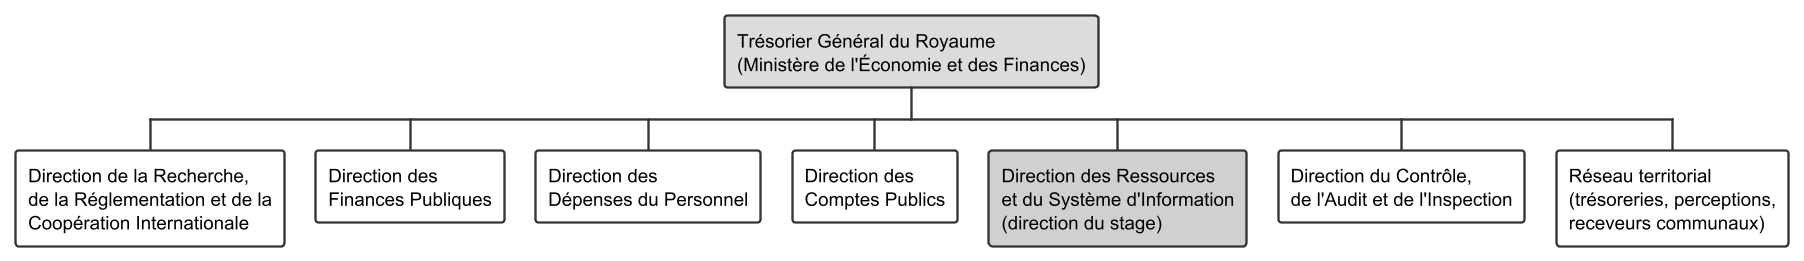
\includegraphics[width=\linewidth]{organigramme.png}
\caption{Organigramme d'ensemble de la Trésorerie Générale du Royaume}
\label{fig:orga}
\end{figure}

Chaque direction se subdivise en divisions, elles-mêmes composées de services
(la structure détaillée figure en annexe~\ref{ann:orga}). Le stage s'est déroulé
au sein de la \textbf{Direction des Ressources et du Système d'Information},
plus précisément dans la \textbf{Division du Développement Informatique}, au sein
du bureau en charge du projet décisionnel (figure~\ref{fig:orgadsi}). Le
stagiaire y a occupé une position de \emph{concepteur-développeur}. Le projet
réalisé s'inscrit pleinement dans les missions de cette division (assistance à la
maîtrise d'ouvrage, architecture, conception et développement) et dans la
dimension \emph{aide à la décision} portée par le bureau d'accueil.

\begin{figure}[H]
\centering
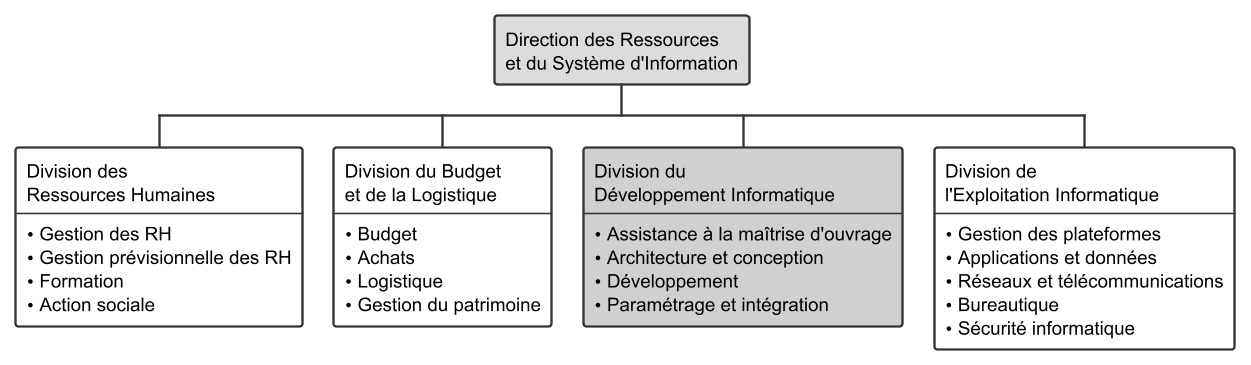
\includegraphics[width=\linewidth]{orga-dsi.png}
\caption{Direction des Ressources et du Système d'Information : divisions et
services (division du stage en grisé)}
\label{fig:orgadsi}
\end{figure}

\noindent\textit{Note.} La présentation de la TGR ci-dessus est réelle. En
revanche, pour des raisons de confidentialité et à des fins pédagogiques, le
corpus réglementaire exploité par l'application (politiques, barèmes, procédures)
est une \textbf{simulation} réaliste et ne reproduit pas des textes officiels de
l'organisme.

\section{Constat et problématique}
La TGR dispose déjà de plusieurs \textbf{outils numériques} permettant de créer
et de gérer les demandes internes ainsi que leurs pièces justificatives.

Le présent projet ne se substitue pas à ces outils : il en constitue une
\textbf{amélioration} par l'ajout d'une couche d'\textbf{intelligence
artificielle} (dialogue en langage naturel, vérification de conformité et
information sourcée). Ce constat conduit à la problématique suivante :

\begin{quote}\itshape
Comment concevoir un système capable d'\textbf{informer} un agent sur ses droits
et procédures, de l'\textbf{assister} dans la formulation de ses demandes en
langage naturel, d'en \textbf{vérifier} automatiquement la conformité au regard
d'un corpus réglementaire, et de ne soumettre à la validation humaine que les
demandes complètes et sourcées, sans se substituer à la décision ?
\end{quote}

\section{Objectifs du projet}
Pour répondre à cette problématique, les objectifs suivants ont été fixés :

\begin{enumerate}
  \item offrir une interface conversationnelle unique (application web
  progressive, poste de travail et mobile) pour \emph{poser des questions} et
  \emph{formuler des demandes} ;
  \item répondre aux questions administratives (congés, missions, frais) à partir
  du corpus réglementaire, avec citation des textes ;
  \item structurer automatiquement chaque demande et détecter les éléments
  manquants (informations et pièces) ;
  \item mettre en place un pipeline RAG indexant un corpus réglementaire français ;
  \item vérifier la conformité et n'acheminer vers la validation que les demandes
  complètes ;
  \item fournir aux responsables un tableau de bord de validation ;
  \item garantir la sécurité (authentification, rôles) et la traçabilité ;
  \item livrer une solution entièrement conteneurisée (Docker).
\end{enumerate}

% =====================================================================
%  CHAPITRE — ÉTAT DE L'ART (revue de littérature)
% =====================================================================
\chapter{État de l'art : LLM, embeddings et RAG}

Ce chapitre situe le projet dans son contexte technologique et scientifique. Il
présente les briques d'intelligence artificielle mobilisées -- grands modèles de
langage, représentations vectorielles, recherche sémantique et génération
augmentée par la recherche -- et explique pourquoi leur combinaison convient à un
assistant administratif \emph{fiable} et \emph{traçable}.

\section{Les grands modèles de langage (LLM)}
Les grands modèles de langage (\emph{Large Language Models}) sont des réseaux de
neurones de type \textbf{Transformer}~\cite{transformer}, entraînés sur
d'immenses corpus textuels à prédire le mot suivant. Ils acquièrent ainsi une
capacité remarquable à comprendre et à produire du langage naturel, à résumer, à
extraire de l'information ou à dialoguer. Deux limites en restreignent toutefois
l'usage administratif direct : ils peuvent \textbf{halluciner}, c'est-à-dire
produire des affirmations plausibles mais fausses ; et leurs connaissances sont
\textbf{figées} à la date de leur entraînement, sans accès aux règlements
internes d'une organisation. Le modèle retenu dans ce projet, \textbf{Qwen3}, est
un LLM multilingue exploité via une API compatible OpenAI.

\section{Les embeddings et la recherche sémantique}
Un \emph{embedding} (plongement) est la représentation d'un texte sous forme de
vecteur numérique de grande dimension, construite de sorte que deux textes de
\emph{sens} proche aient des vecteurs proches, au sens d'une distance (ici le
cosinus)~\cite{sbert}. Cette propriété autorise une \textbf{recherche
sémantique} : plutôt que de chercher des mots-clés exacts, on encode la question
et l'on récupère les passages dont le vecteur est le plus proche
(figure~\ref{fig:embed}). Le projet emploie le modèle multilingue
\textbf{bge-m3}~\cite{bgem3}, performant sur le français, qui produit des vecteurs
de 1024 dimensions.

\begin{figure}[H]
\centering
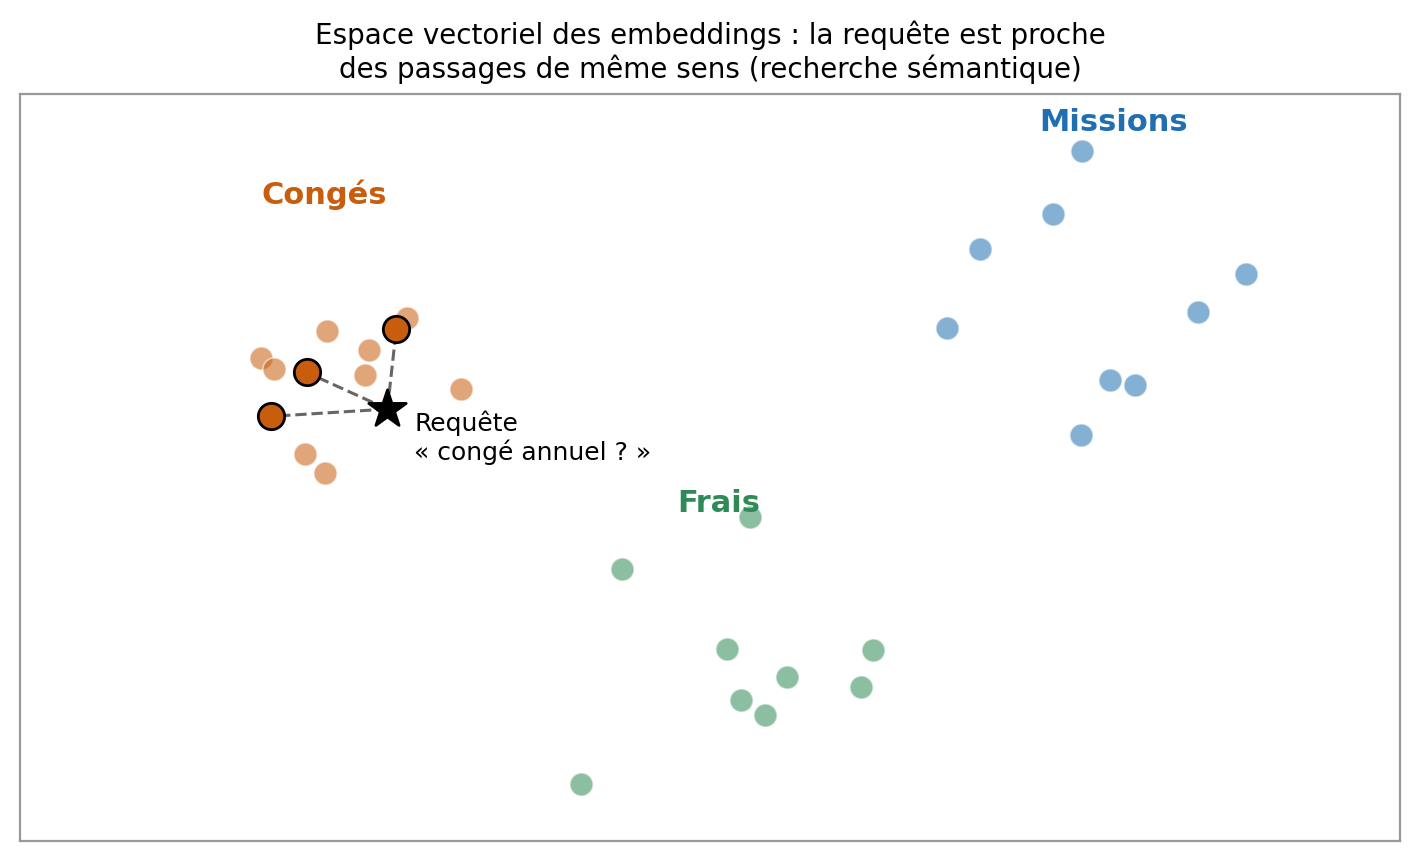
\includegraphics[width=0.82\linewidth]{embeddings-space.png}
\caption{Principe de la recherche sémantique dans l'espace des embeddings}
\label{fig:embed}
\end{figure}

\section{Les bases de données vectorielles}
Stocker et interroger efficacement de nombreux vecteurs suppose un index
spécialisé pour la recherche approchée des plus proches voisins. Plutôt que
d'ajouter une base vectorielle dédiée, le projet s'appuie sur
\textbf{pgvector}~\cite{pgvector}, une extension de PostgreSQL qui apporte un type
\texttt{vector} et des index de similarité directement dans le système de gestion
de base de données relationnel déjà utilisé -- simplifiant ainsi l'architecture.

\section{La génération augmentée par la recherche (RAG)}
La \textbf{génération augmentée par la recherche} (\emph{Retrieval-Augmented
Generation}), introduite par Lewis \emph{et al.}~\cite{rag}, associe un module de
\textbf{recherche} et un module de \textbf{génération} : à chaque question, on
récupère d'abord les passages pertinents d'un corpus de référence, puis on les
fournit au LLM comme contexte pour qu'il formule sa réponse. Cette approche
répond directement aux deux limites des LLM : elle \textbf{ancre} les réponses
dans des sources vérifiables -- réduisant les hallucinations -- et permet
d'exploiter des connaissances \textbf{à jour et privées} (les règlements
internes) sans réentraîner le modèle. Elle rend en outre les réponses
\textbf{traçables} par citation des textes, exigence forte en contexte
administratif. La mise en oeuvre détaillée est présentée au
chapitre~\ref{chap:ia}.

\section{Positionnement du projet}
Le projet applique ces techniques à un cas métier concret : un assistant qui,
au lieu de répondre « en général », s'appuie sur le corpus réglementaire de
l'organisation pour \emph{informer} l'agent et \emph{vérifier} la conformité de
ses demandes, tout en laissant la décision finale à un responsable humain. Il se
distingue ainsi d'un simple agent conversationnel par sa \textbf{fiabilité} (RAG,
citations) et son \textbf{intégration métier} (création et validation de
demandes).

% =====================================================================
%  CHAPITRE 2
% =====================================================================
\chapter{Étude et conception}

\section{Solution proposée}
La solution se compose de trois applications reposant sur une API unique : une
\textbf{application web progressive} (accessible sur poste de travail comme sur
mobile) pour l'employé, un \textbf{tableau de bord web} pour les responsables, et
un \textbf{backend} hébergeant l'API REST, l'orchestrateur IA et le pipeline RAG.

\section{Acteurs et rôles}
Le système distingue trois rôles utilisateurs et un acteur logiciel
(l'assistant IA), décrits au tableau~\ref{tab:acteurs}. La validation n'est pas
hiérarchisée : plusieurs \emph{responsables} peuvent statuer sur les demandes.

\begin{table}[H]
\centering
\begin{tabularx}{\linewidth}{>{\bfseries}l X}
\toprule
\rowcolor{gHead}\thd{Acteur} & \thd{Responsabilités} \\
\midrule
Employé & Pose des questions administratives, formule ses demandes via
l'assistant, consulte son solde de congés, suit et modifie ses demandes. \\
\rowcolor{gBand}
Responsable & Consulte la file des demandes et l'analyse de conformité, décide
(approuver, rejeter, demander des modifications), interroge l'IA. \\
Administrateur & Gère la base de connaissances, consulte l'annuaire et le
journal d'audit. \\
\rowcolor{gBand}
Assistant IA & Répond aux questions (RAG), détecte l'intention, extrait les
informations, vérifie la conformité et explique (citations). \\
\bottomrule
\end{tabularx}
\caption{Acteurs du système et leurs responsabilités}
\label{tab:acteurs}
\end{table}

\section{Diagramme de cas d'utilisation}
La figure~\ref{fig:uc} synthétise les fonctionnalités offertes à chaque acteur
ainsi que les traitements internes de l'IA (relations \emph{include} et
\emph{extend}).

\begin{sidewaysfigure}
\centering
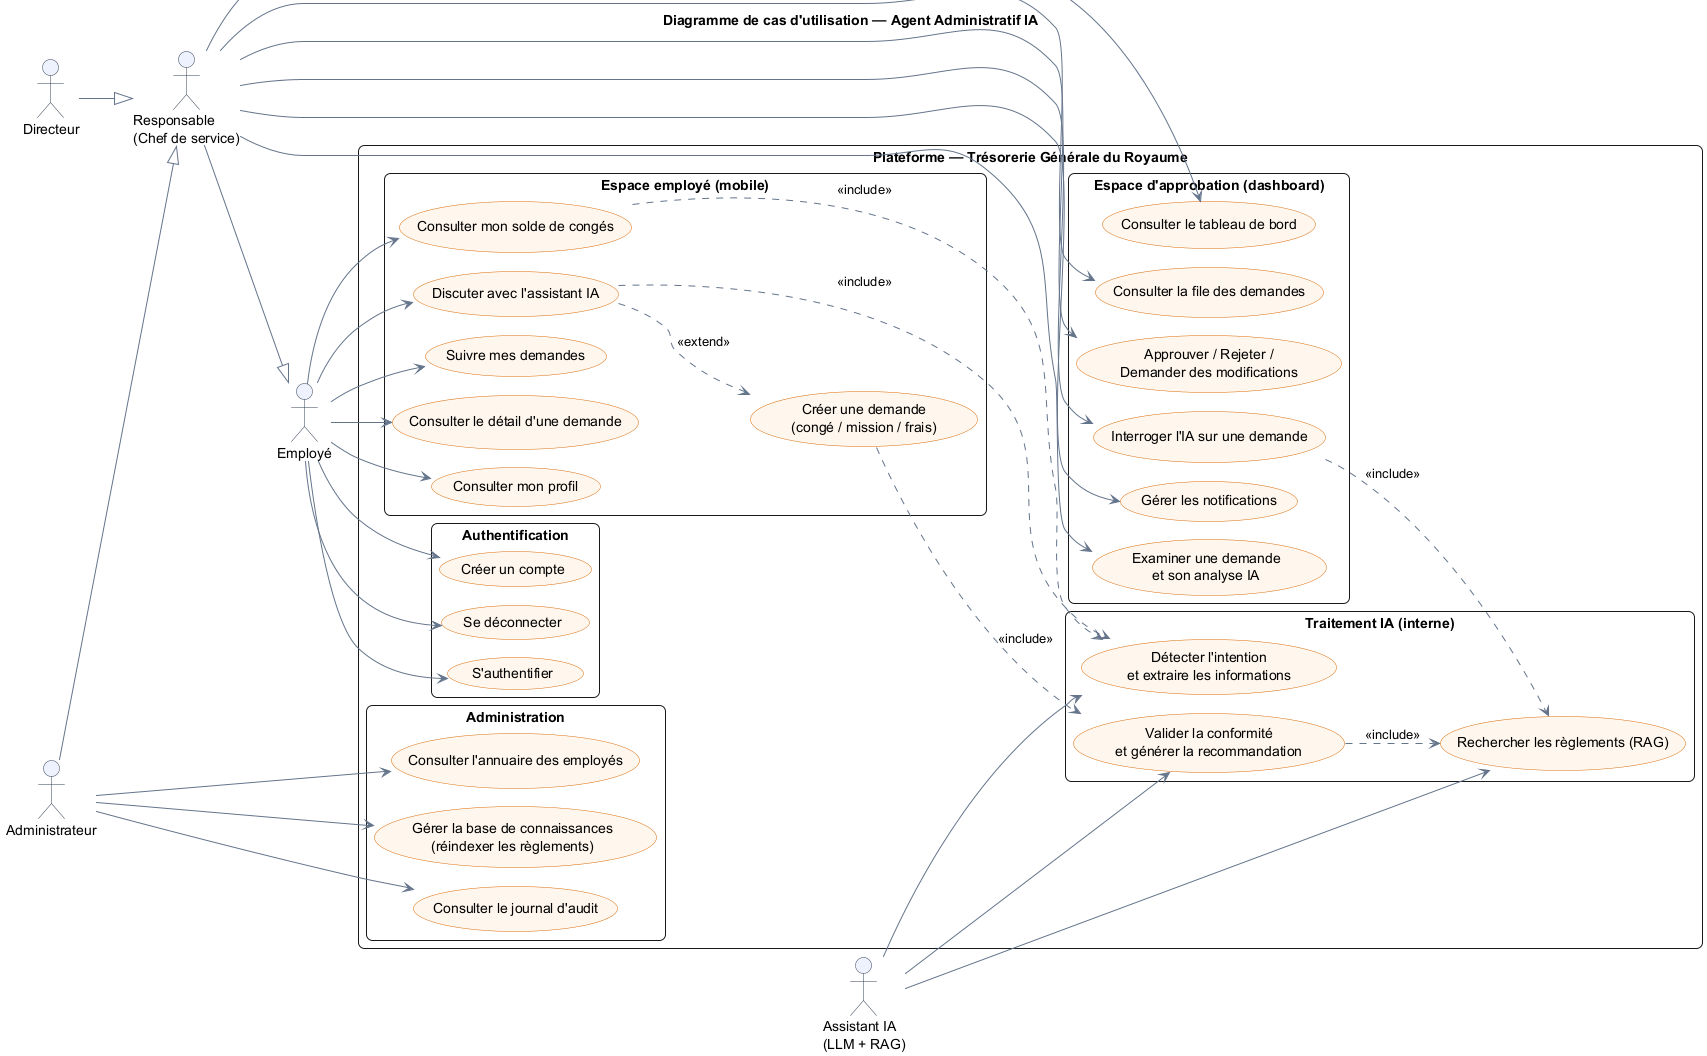
\includegraphics[width=0.92\textheight,height=0.95\textwidth,keepaspectratio]{UC.png}
\caption{Diagramme de cas d'utilisation}
\label{fig:uc}
\end{sidewaysfigure}

\section{Modèle du domaine}
Le modèle de données (figure~\ref{fig:classes}) comporte douze entités
persistantes. La demande administrative est centrale : ses champs spécifiques au
type (dates, montants, destination) sont stockés dans une colonne \texttt{JSONB}
alimentée par l'IA, ce qui évite un schéma rigide par type de demande.

\begin{sidewaysfigure}
\centering
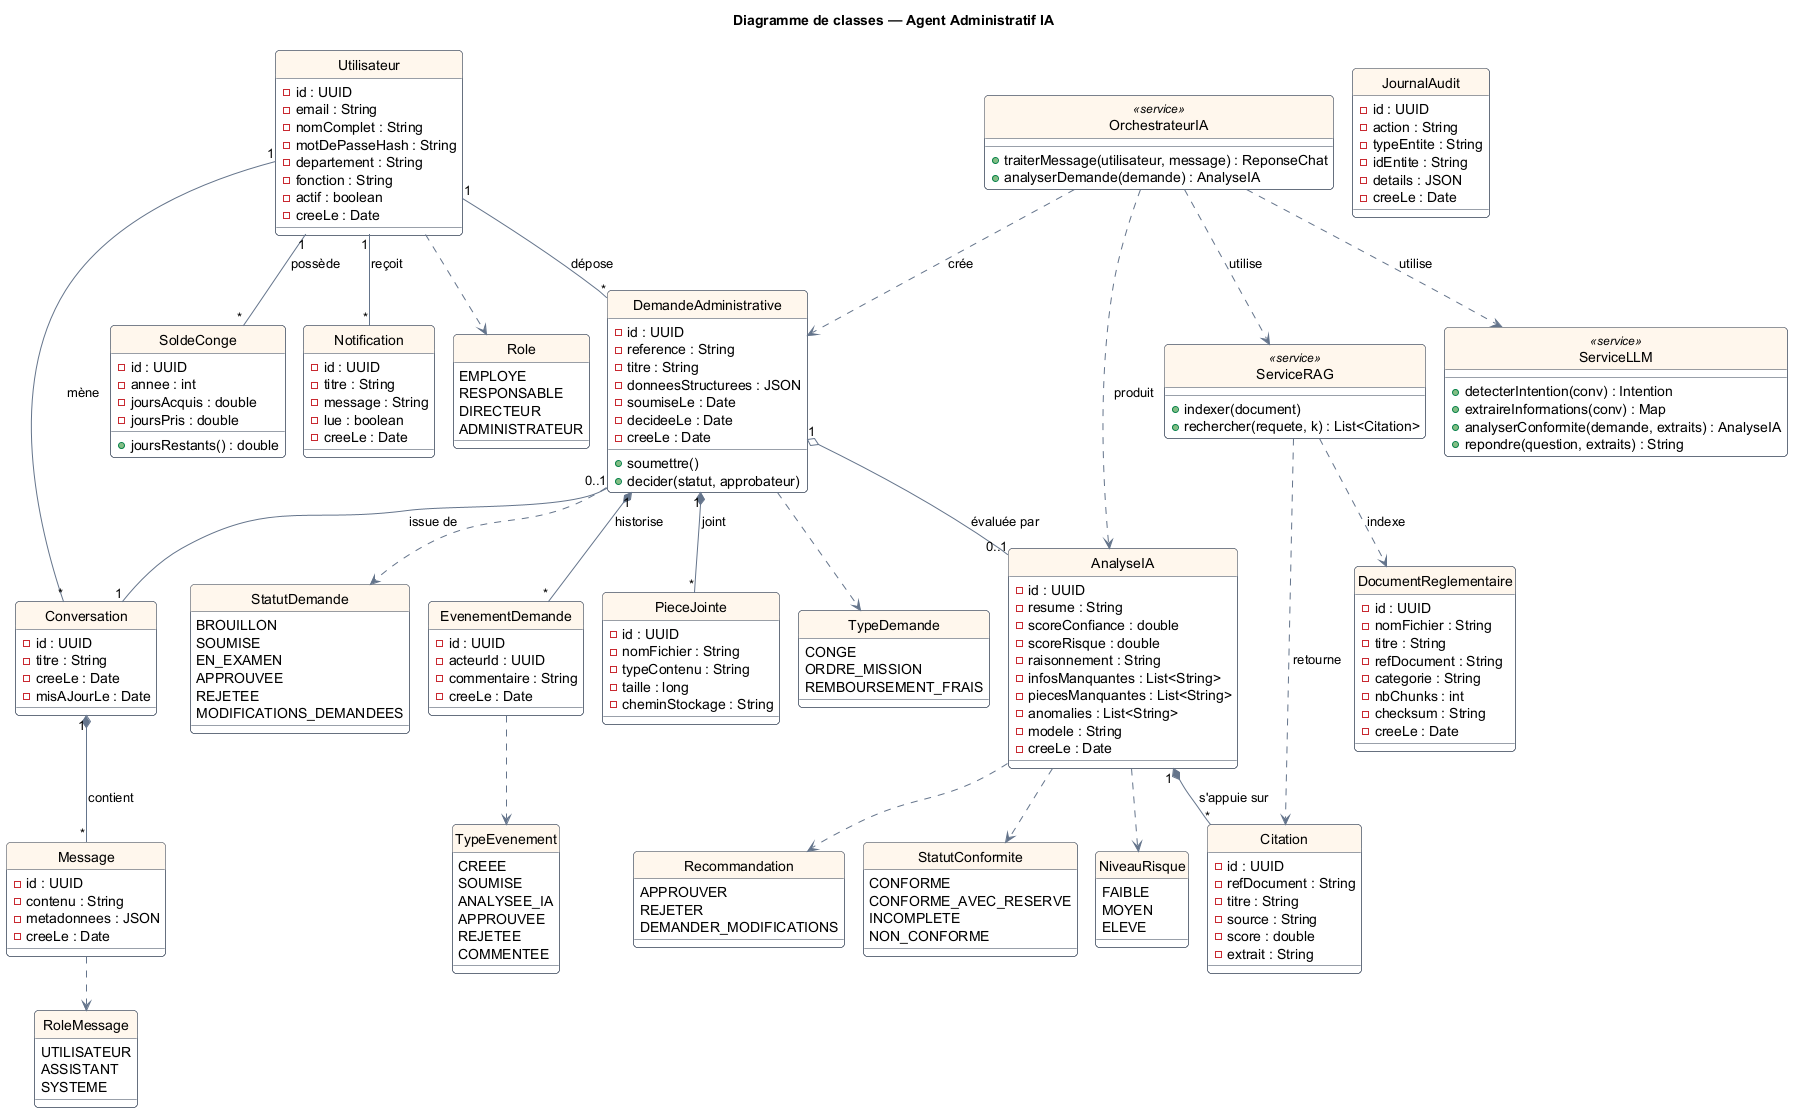
\includegraphics[width=0.92\textheight,height=0.95\textwidth,keepaspectratio]{Classe.png}
\caption{Diagramme de classes du domaine}
\label{fig:classes}
\end{sidewaysfigure}

\section{Diagramme de séquence}
La figure~\ref{fig:seq} illustre le scénario nominal : création d'une demande de
congé via l'assistant (dialogue, extraction, création), analyse de conformité
(RAG puis LLM), et validation humaine sur le tableau de bord.

\begin{figure}[p]
\centering
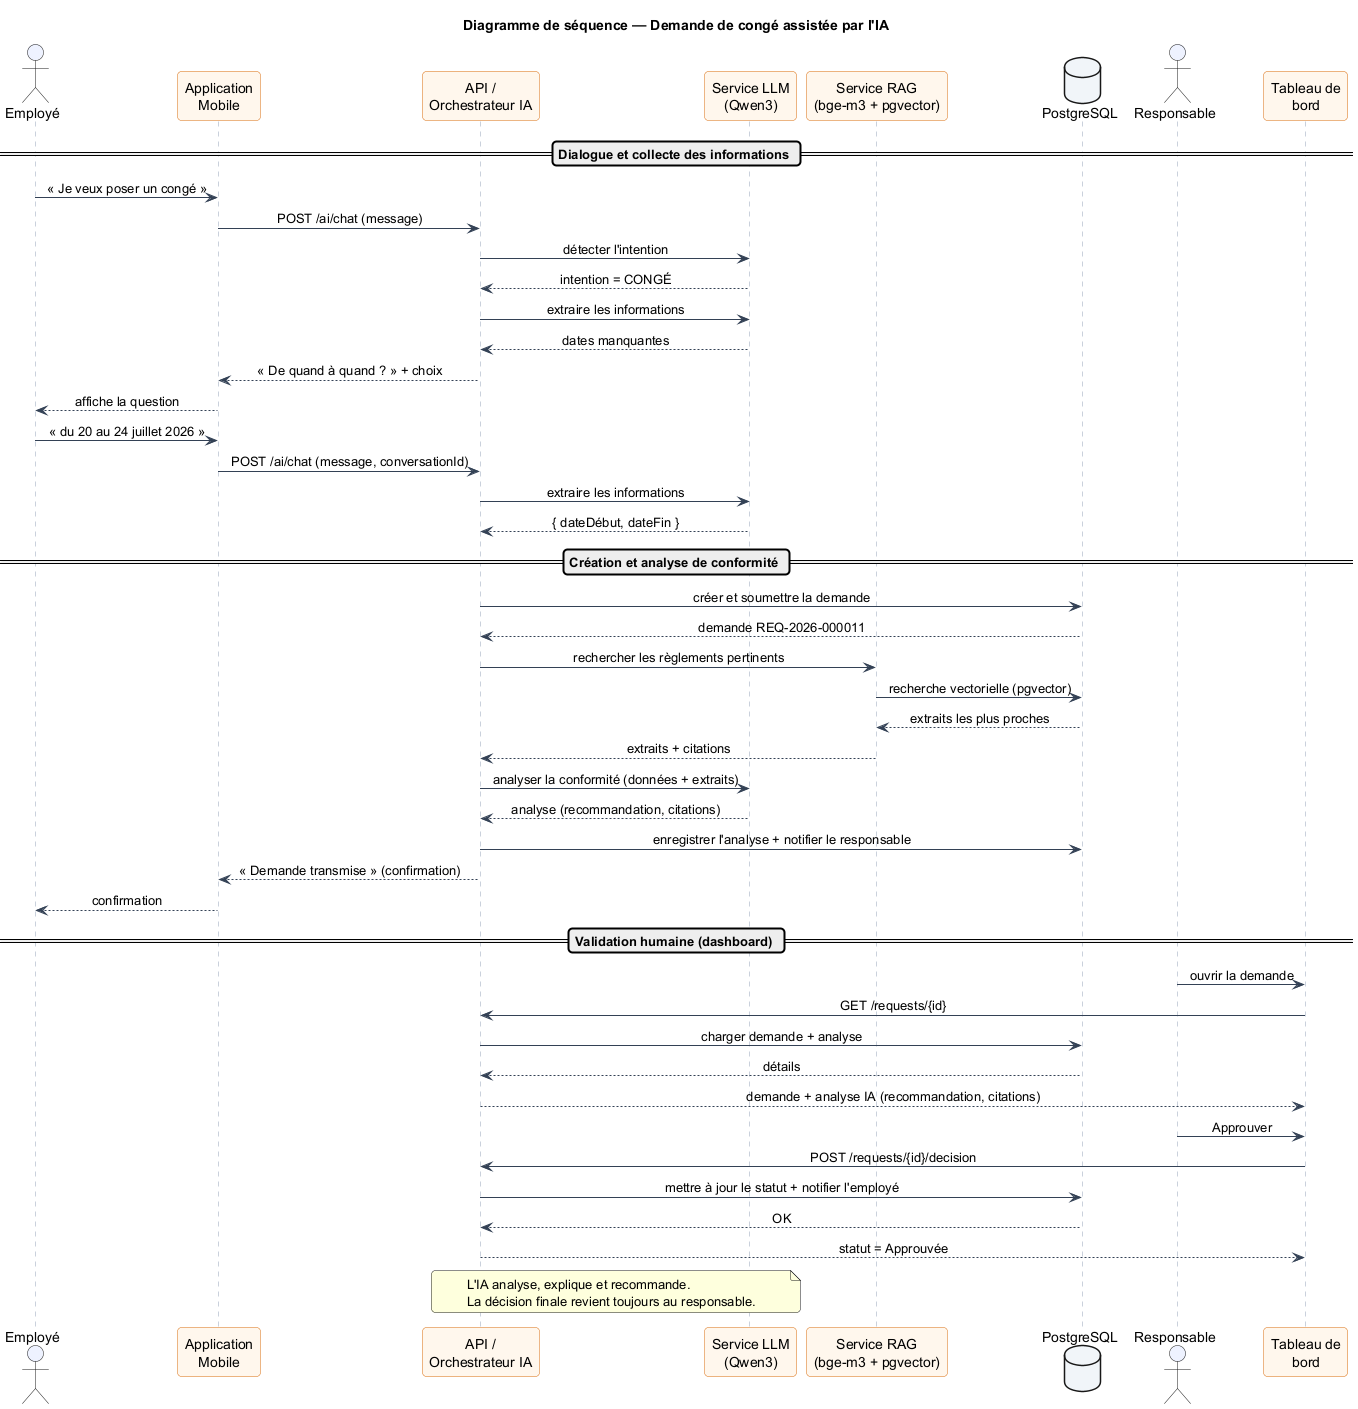
\includegraphics[width=\linewidth,height=0.92\textheight,keepaspectratio]{Sequence.png}
\caption{Diagramme de séquence : demande assistée puis validation}
\label{fig:seq}
\end{figure}

% =====================================================================
%  CHAPITRE 3
% =====================================================================
\chapter{Architecture technique}

\section{Vue d'ensemble}
L'architecture (figure~\ref{fig:archi}) adopte un découpage en couches et une
organisation \emph{par fonctionnalité} côté backend. Les clients communiquent
avec le backend via une API REST sécurisée par JWT. Le backend s'appuie sur
PostgreSQL (données métier \emph{et} vecteurs, grâce à pgvector), sur Ollama pour
le calcul des embeddings, et sur un LLM distant exposé via une API compatible
OpenAI.

\begin{figure}[H]
\centering
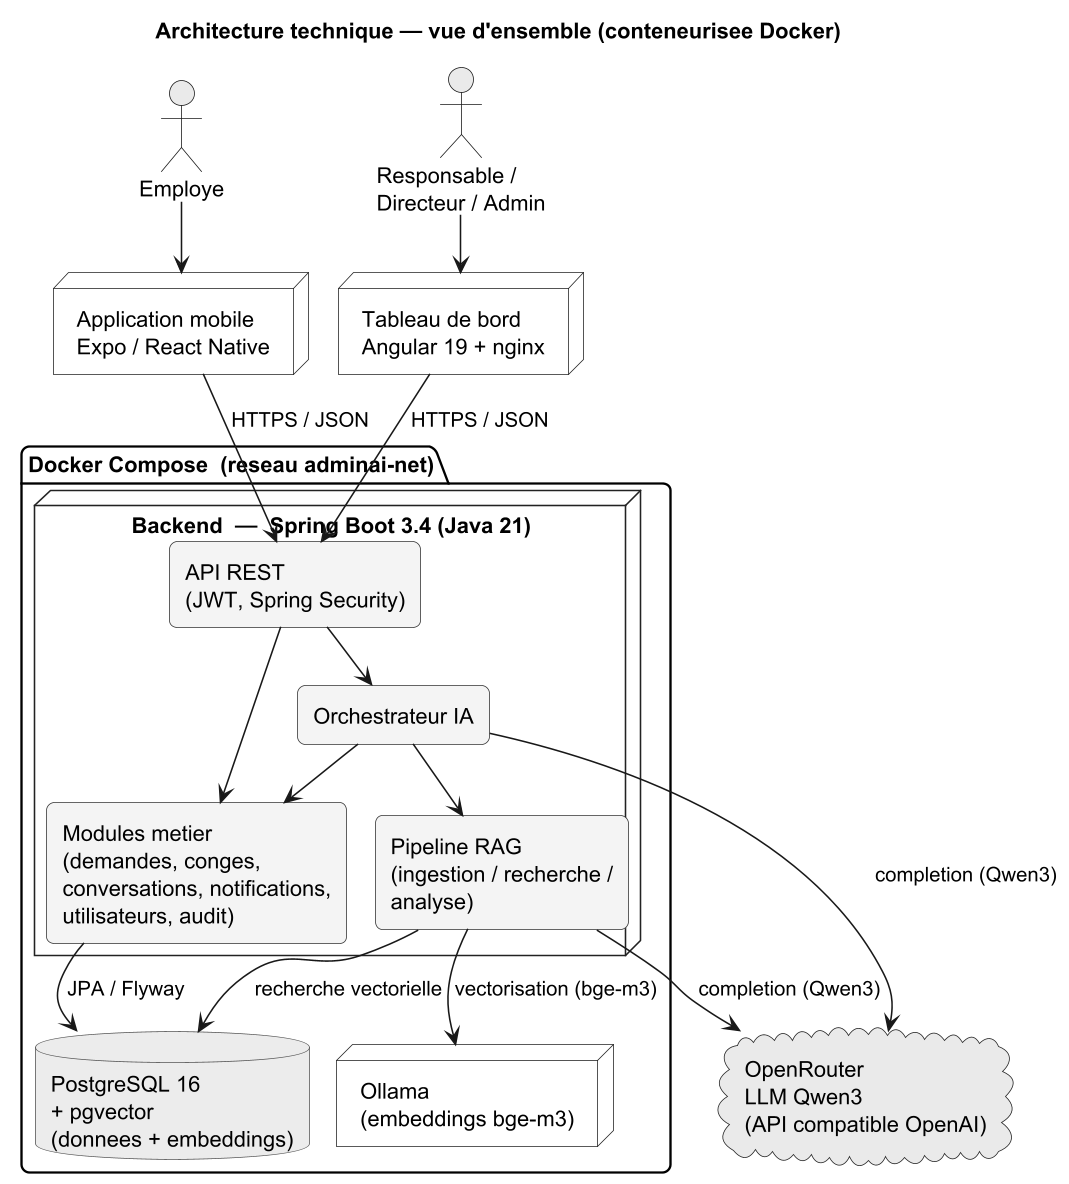
\includegraphics[width=0.94\linewidth]{architecture.png}
\caption{Architecture technique conteneurisée}
\label{fig:archi}
\end{figure}

\section{Pile technologique}
Le tableau~\ref{tab:stack} récapitule les principales technologies retenues,
parmi lesquelles Spring Boot~\cite{springboot}, LangChain4j~\cite{langchain4j},
Angular~\cite{angular}, Expo~\cite{expo} et Docker~\cite{docker}, toutes
largement éprouvées et documentées.

\begin{table}[H]
\centering\small
\setlength{\tabcolsep}{5pt}
\renewcommand{\arraystretch}{1.55}
\begin{tabularx}{\linewidth}{@{}>{\centering\arraybackslash}m{2.35cm} >{\bfseries}l l >{\raggedright\arraybackslash}X@{}}
\toprule
\rowcolor{gHead}\thd{Logos} & \thd{Couche} & \thd{Technologie} & \thd{Rôle} \\
\midrule
\tlogo{java.pdf}\,\tlogo{spring.pdf} & Backend & Spring Boot 3.4 (Java 21) & API REST, sécurité, orchestration. \\
\rowcolor{gBand}
\tlogo{springsec.pdf}\,\tlogo{jwt.pdf} & Sécurité & Spring Security + JWT & Authentification stateless, rôles. \\
\tlogo{spring.pdf} & Persistance & Spring Data JPA + Flyway & ORM et migrations versionnées. \\
\rowcolor{gBand}
\tlogo{postgresql.pdf} & Base de données & PostgreSQL 16 + pgvector & Données métier et vecteurs. \\
\tlogo{langchain.pdf}\,\tlogo{apache.pdf} & IA / RAG & LangChain4j & Abstraction LLM, embeddings, pgvector, Tika. \\
\rowcolor{gBand}
\tlogo{qwen.pdf}\,\tlogo{openrouter.pdf} & LLM & Qwen3 (via OpenRouter) & Génération, API compatible OpenAI. \\
\tlogo{huggingface.pdf}\,\tlogo{ollama.pdf} & Embeddings & bge-m3 / Ollama & Vectorisation locale des textes. \\
\rowcolor{gBand}
\tlogo{angular.pdf}\,\tlogo{tailwind.pdf} & Dashboard & Angular 19 + Tailwind & Application monopage, servie par nginx. \\
\tlogo{expo.pdf}\,\tlogo{react.pdf} & Application employé & Expo / React Native & Web progressif : navigateur et mobile. \\
\rowcolor{gBand}
\tlogo{docker.pdf}\,\tlogo{nginx.pdf} & Conteneurisation & Docker Compose & Orchestration des services (nginx). \\
\bottomrule
\end{tabularx}
\caption{Pile technologique du projet et logos associés}
\label{tab:stack}
\end{table}

\section{Justification des principaux choix}
\begin{itemize}
  \item \textbf{PostgreSQL + pgvector} : un seul moteur pour les données métier
  et les vecteurs simplifie l'exploitation et évite une base vectorielle dédiée.
  \item \textbf{LangChain4j} : abstractions homogènes (chat, embeddings, magasin
  de vecteurs, découpeur) isolant le code métier des API des fournisseurs.
  \item \textbf{Embeddings locaux (bge-m3)} : modèle multilingue performant sur
  le français, exécuté localement (maîtrise des coûts et des données).
  \item \textbf{LLM via API compatible OpenAI} : fournisseur et modèle
  interchangeables par simple configuration.
\end{itemize}

\section{Conteneurisation}
L'infrastructure est décrite dans un fichier \texttt{docker-compose.yml}
orchestrant cinq services (tableau~\ref{tab:docker}). La figure~\ref{fig:docker}
montre la pile en cours d'exécution.

\begin{table}[H]
\centering
\begin{tabularx}{\linewidth}{>{\bfseries}l X}
\toprule
\rowcolor{gHead}\thd{Service} & \thd{Rôle} \\
\midrule
postgres & PostgreSQL 16 + pgvector ; extensions activées à l'initialisation. \\
\rowcolor{gBand}
ollama & Serveur d'inférence local pour le modèle d'embeddings. \\
ollama-init & Tâche unique qui télécharge le modèle bge-m3 puis s'arrête. \\
\rowcolor{gBand}
backend & API Spring Boot ; montage de la base de connaissances en lecture seule. \\
dashboard & Application Angular servie par nginx. \\
\bottomrule
\end{tabularx}
\caption{Services Docker Compose}
\label{tab:docker}
\end{table}

\begin{figure}[H]
\centering
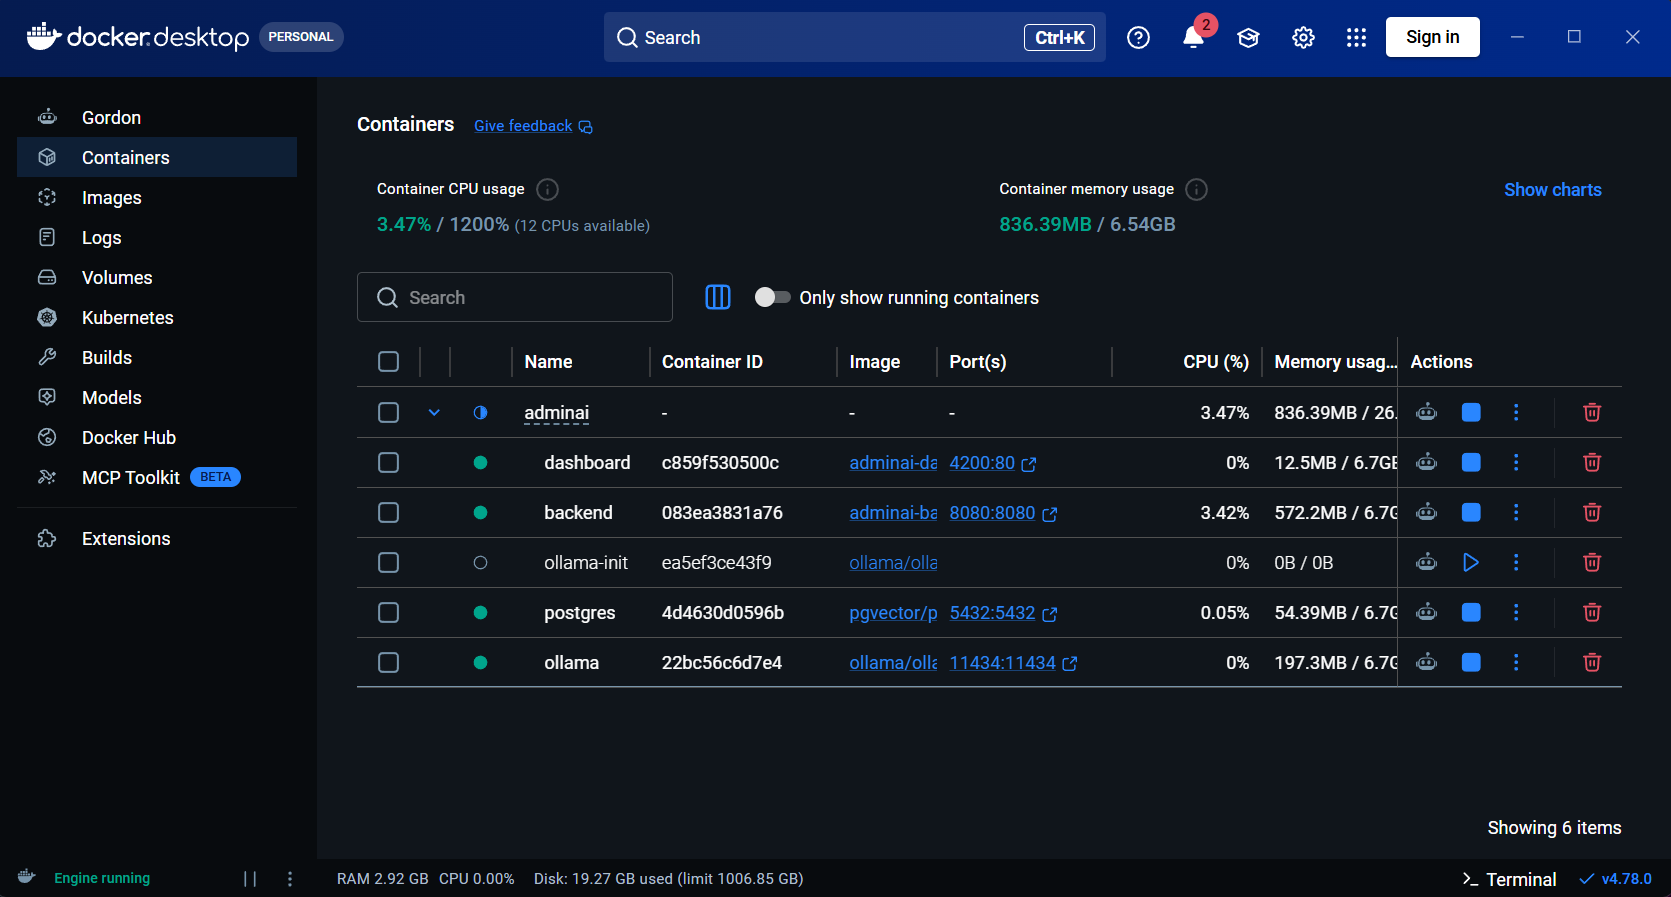
\includegraphics[width=0.95\linewidth]{docker-containers.png}
\caption{Pile applicative conteneurisée en cours d'exécution}
\label{fig:docker}
\end{figure}

% =====================================================================
%  CHAPITRE 4
% =====================================================================
\chapter{Intégration de l'intelligence artificielle}
\label{chap:ia}

Le coeur du projet repose sur un pipeline de génération augmentée par la
recherche (RAG). Le principe consiste à \textbf{ancrer} les réponses du modèle
dans un corpus de référence, afin de réduire les hallucinations et de fournir des
citations vérifiables.

\section{Vue d'ensemble du pipeline}
Le pipeline (figure~\ref{fig:rag}) comprend une phase hors ligne (ingestion du
corpus) et une phase en ligne (interrogation).

\begin{figure}[H]
\centering
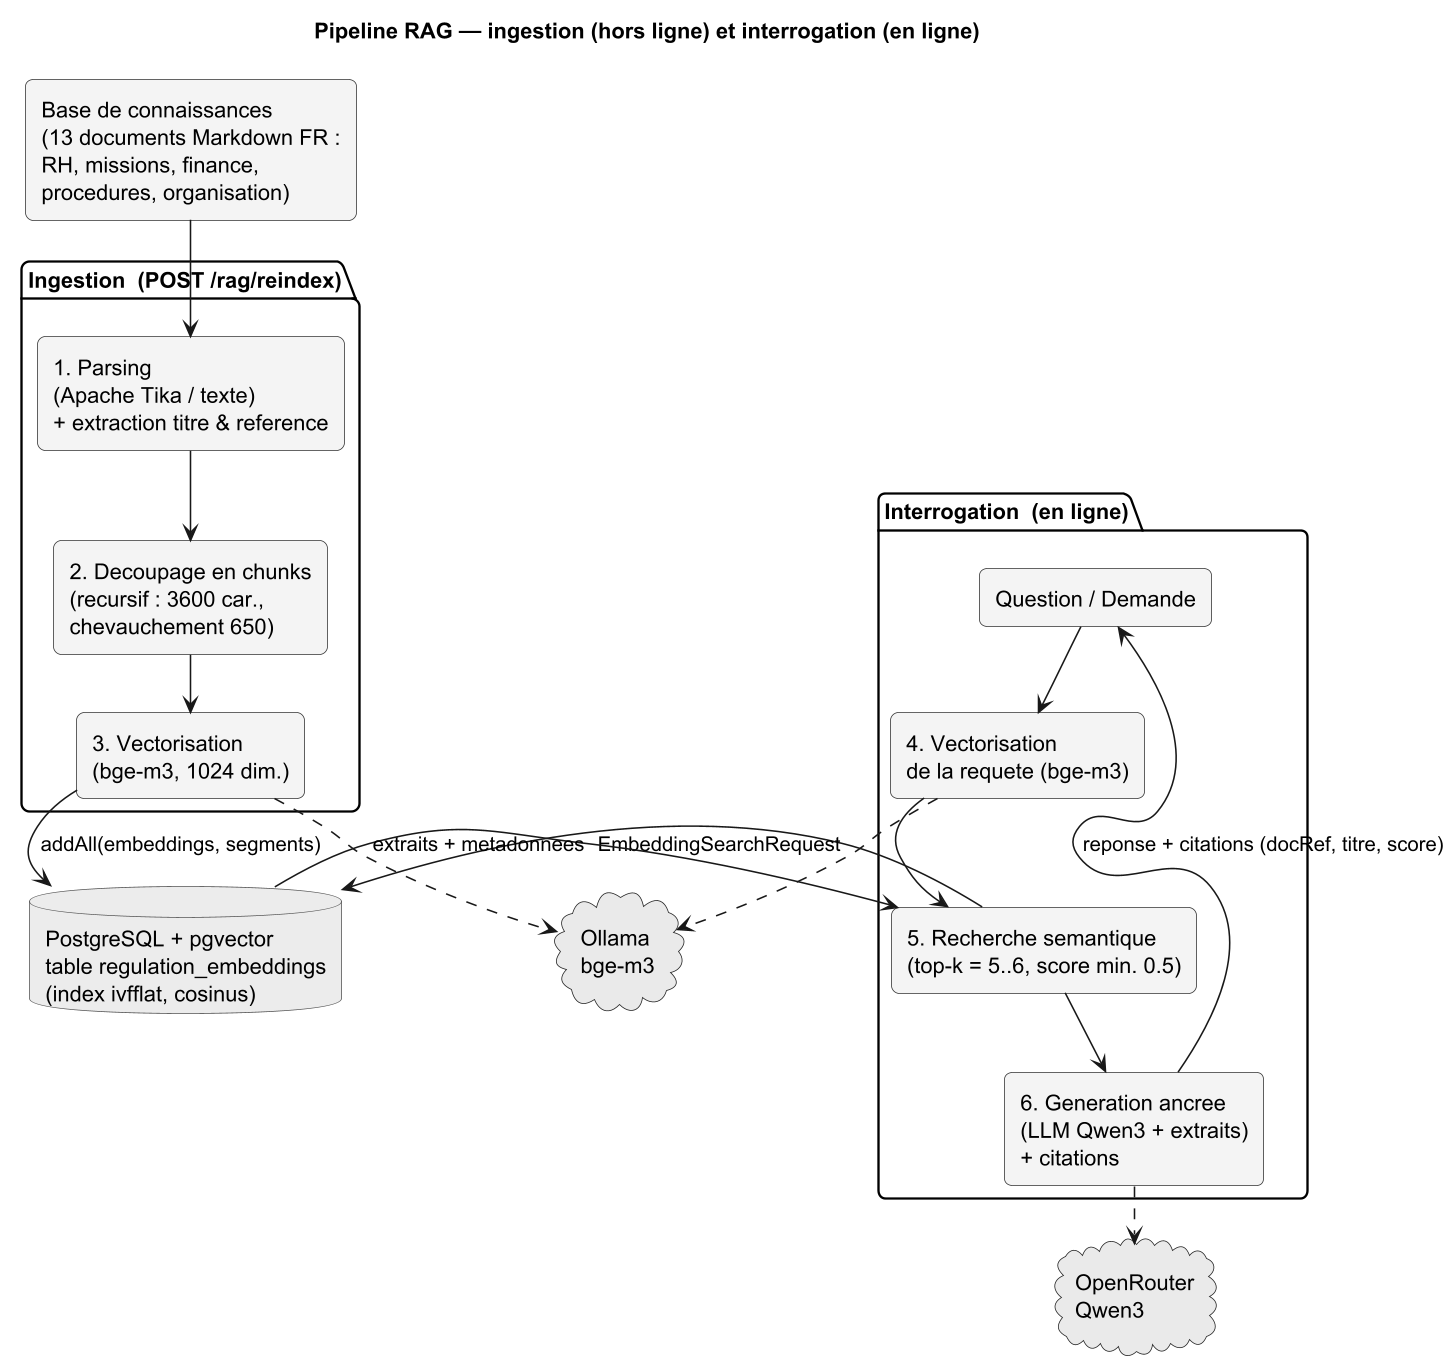
\includegraphics[width=0.95\linewidth]{rag-pipeline.png}
\caption{Pipeline RAG : ingestion et interrogation}
\label{fig:rag}
\end{figure}

\section{Ingestion : analyse, découpage, vectorisation}
L'ingestion est déclenchée par un point d'entrée réservé à l'administrateur.
Pour chaque document du corpus (treize documents Markdown en français) :

\begin{enumerate}
  \item \textbf{analyse} du contenu (Apache Tika pour les formats binaires) et
  extraction du titre et de la référence documentaire ;
  \item \textbf{idempotence} par condensé SHA-256 (un document identique n'est
  pas réindexé) ;
  \item \textbf{découpage} récursif en fragments de 3600 caractères avec 650
  caractères de chevauchement ;
  \item \textbf{vectorisation} de chaque fragment par bge-m3 (1024 dimensions) ;
  \item \textbf{stockage} des vecteurs et de leurs métadonnées de citation dans
  la table pgvector (index de similarité, distance cosinus).
\end{enumerate}

\section{Recherche sémantique}
À l'interrogation, la requête est encodée par le même modèle, puis une recherche
des plus proches voisins est menée dans pgvector. Deux garde-fous sont
appliqués : un nombre maximal de résultats et un score minimal de similarité,
qui écarte les extraits peu pertinents. Chaque résultat conserve ses métadonnées,
ce qui permet de construire des citations traçables.

\section{Orchestration et analyse explicable}
L'orchestrateur détecte l'intention du message puis aiguille le traitement :
question administrative (questions-réponses par RAG), consultation de solde, ou
création d'une demande. Le traitement d'une demande suit une logique
\emph{demander puis soumettre} : extraction des informations, contrôle des dates
(toute date passée est refusée), demande unique des éléments manquants, collecte
des pièces justificatives, puis soumission.

Une fois la demande soumise, le service d'analyse produit une évaluation
explicable : il récupère les règlements pertinents (RAG), demande au LLM une
validation structurée (statut de conformité, niveau de risque, recommandation,
anomalies, raisonnement), puis persiste l'analyse avec ses citations. Point
essentiel pour la fiabilité : les informations et pièces manquantes sont
\textbf{calculées de manière déterministe} à partir de ce que l'employé a
réellement fourni, et non laissées à l'appréciation du modèle. La décision finale
demeure exclusivement humaine.

\par\noindent\begin{minipage}{\linewidth}
\begin{lstlisting}[language=Java,caption={Aiguillage par intention (orchestrateur)}]
ChatResponse response = switch (intent) {
    case SMALL_TALK     -> smallTalk(convId, message);
    case ADMIN_QUESTION -> answerQuestion(convId, message);   // Q&R via RAG
    case BALANCE_QUERY  -> handleBalance(userId, convId, message);
    case LEAVE, MISSION_ORDER, EXPENSE
                        -> handleRequest(userId, convId, intent, transcript, alreadyAsked);
};
\end{lstlisting}
\end{minipage}

% =====================================================================
%  CHAPITRE 5
% =====================================================================
\chapter{Réalisation et déroulement du stage}

\section{Méthodologie de travail}
Le travail a été conduit de manière itérative et incrémentale : chaque
fonctionnalité était conçue, développée, puis vérifiée de bout en bout avant de
passer à la suivante. L'environnement conteneurisé a permis de reproduire, en
local, une pile proche de la production (base de données, moteur d'embeddings,
API). Les étapes principales ont été : mise en place de l'infrastructure et de la
sécurité, construction du pipeline RAG, développement de l'orchestrateur IA, puis
réalisation des interfaces (application web progressive et tableau de bord).

\section{Modules du backend et API}
Le backend est organisé par fonctionnalité ; chaque module regroupe son domaine,
son dépôt, son service et sa couche web. Le tableau~\ref{tab:api} recense les
principaux points d'entrée de l'API et les accès associés.

\begin{table}[H]
\centering\small\setlength{\tabcolsep}{5pt}
\begin{tabular}{l l l}
\toprule
\rowcolor{gHead}\thd{Méthode et chemin} & \thd{Fonction} & \thd{Accès} \\
\midrule
\ttfamily POST /auth/login & Connexion & Public \\
\rowcolor{gBand}
\ttfamily POST /ai/chat & Dialoguer avec l'assistant & Authentifié \\
\ttfamily POST /ai/ask & Question administrative (RAG) & Authentifié \\
\rowcolor{gBand}
\ttfamily POST /requests & Créer une demande & Authentifié \\
\ttfamily GET /requests/mine & Mes demandes & Authentifié \\
\rowcolor{gBand}
\ttfamily POST /requests/\{id\}/attachments & Joindre une pièce & Authentifié \\
\ttfamily GET /requests/pending & File des demandes en attente & Approbateur \\
\rowcolor{gBand}
\ttfamily GET /requests/stats & Statistiques & Approbateur \\
\ttfamily POST /requests/\{id\}/decision & Décider & Responsable \\
\rowcolor{gBand}
\ttfamily GET /leave-balances/me & Mon solde de congés & Authentifié \\
\ttfamily GET /users & Annuaire des employés & Approbateur \\
\rowcolor{gBand}
\ttfamily POST /rag/reindex & Réindexer la base de connaissances & Admin \\
\ttfamily GET /audit & Journal d'audit & Admin \\
\bottomrule
\end{tabular}
\caption{Principaux points d'entrée de l'API REST}
\label{tab:api}
\end{table}

\section{Application de l'employé (web progressive)}
L'application de l'employé est une \textbf{application web progressive} (PWA)
utilisable indifféremment depuis un navigateur de poste de travail ou un mobile.
Elle s'organise autour d'une barre d'onglets : \textbf{Accueil},
\textbf{Assistant}, \textbf{Demandes} et \textbf{Profil}. Les écrans sont
présentés ci-dessous dans l'ordre du parcours d'un utilisateur.

Un nouvel agent commence par \textbf{créer son compte}
(figure~\ref{fig:minscription}), en renseignant son identité et sa direction de
rattachement.

\begin{figure}[H]
\centering
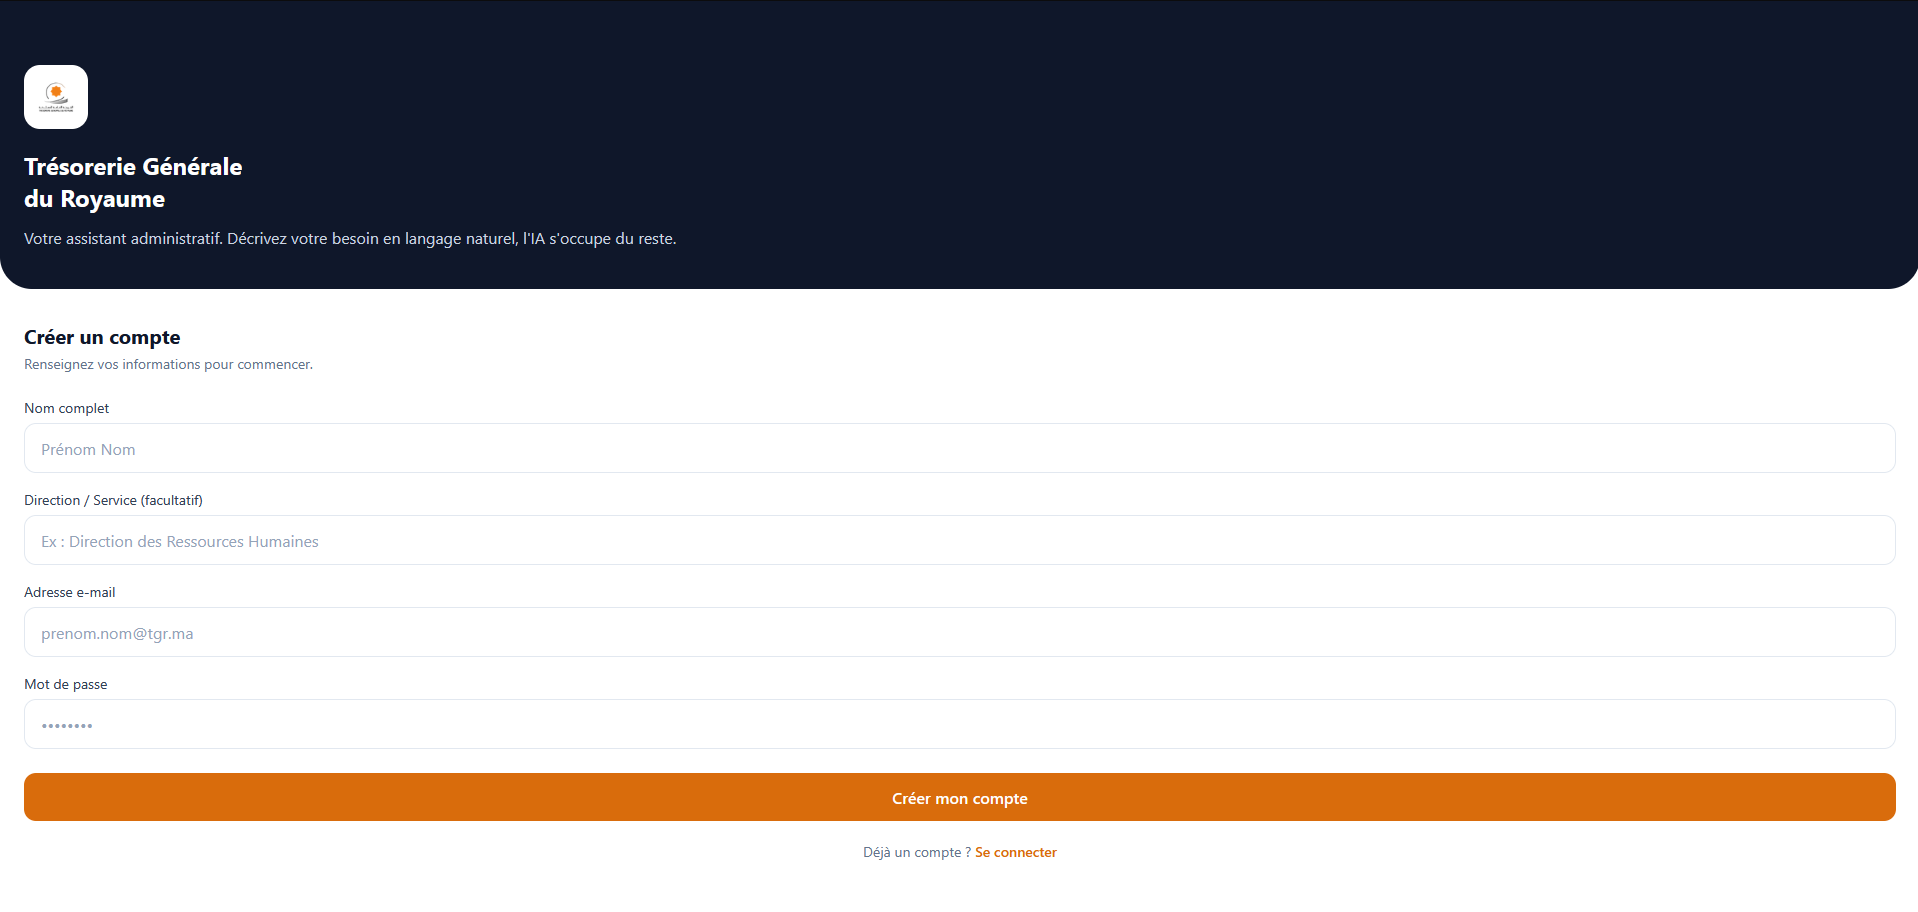
\includegraphics[width=0.86\linewidth]{mobile-inscription.png}
\caption{Application employé : création de compte}
\label{fig:minscription}
\end{figure}

Il se \textbf{connecte} ensuite (figure~\ref{fig:mconnexion}) ; la session est
conservée entre les rechargements et n'est fermée qu'à la déconnexion.

\begin{figure}[H]
\centering

\includegraphics[width=0.86\linewidth]{mobile-connexion.png}
\caption{Application employé : écran de connexion}
\label{fig:mconnexion}
\end{figure}

L'\textbf{écran d'accueil} (figure~\ref{fig:maccueil}) affiche le solde de congés,
les actions principales et les demandes récentes.

\begin{figure}[H]
\centering
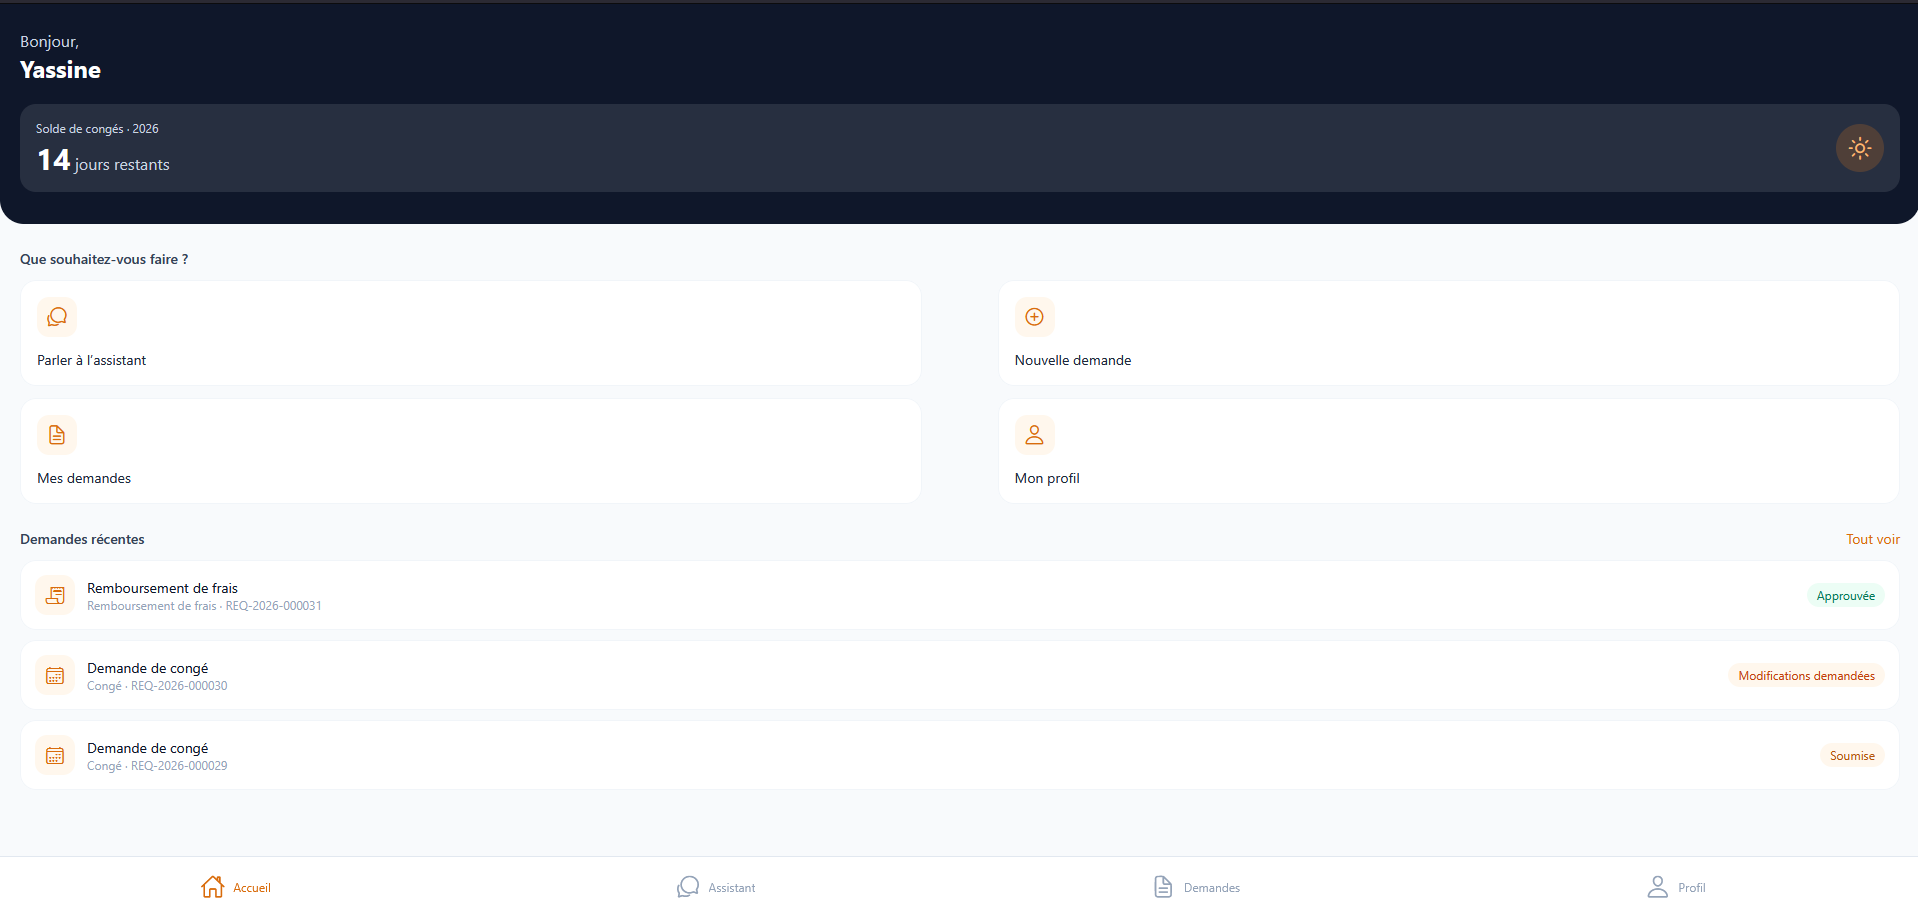
\includegraphics[width=0.86\linewidth]{mobile-accueil.png}
\caption{Application employé : page d'accueil}
\label{fig:maccueil}
\end{figure}

À l'ouverture de l'\textbf{assistant} (figure~\ref{fig:mentree}), l'agent choisit
entre les deux fonctions du système -- \emph{soumettre une demande} ou
\emph{obtenir une information} --, ce qui matérialise le double rôle de l'outil :
guichet de demandes et fournisseur d'informations administratives sourcées.

\begin{figure}[H]
\centering
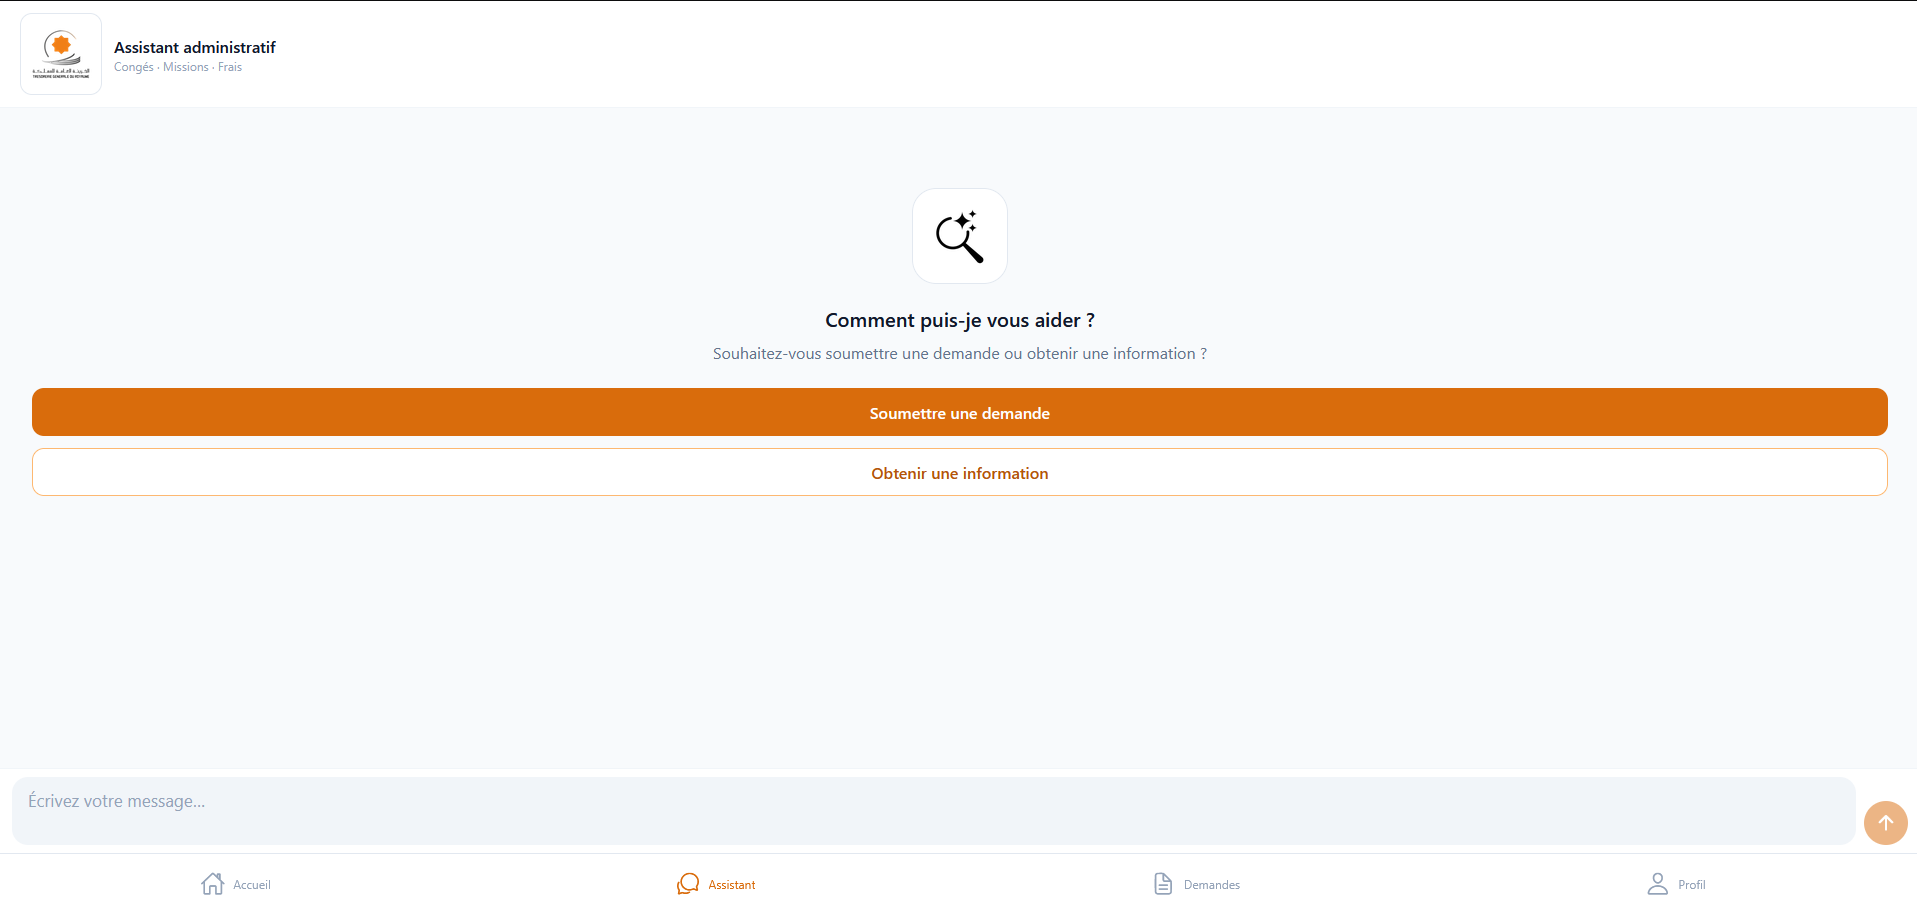
\includegraphics[width=0.86\linewidth]{assistant-entree.png}
\caption{Application employé : assistant (écran d'accueil, avant le dialogue)}
\label{fig:mentree}
\end{figure}

Le dialogue s'engage alors en langage naturel (figure~\ref{fig:massistant}) : les
réponses de l'IA peuvent proposer des choix tactiles, et un panneau permet de
joindre les pièces justificatives avant l'envoi.

\begin{figure}[H]
\centering
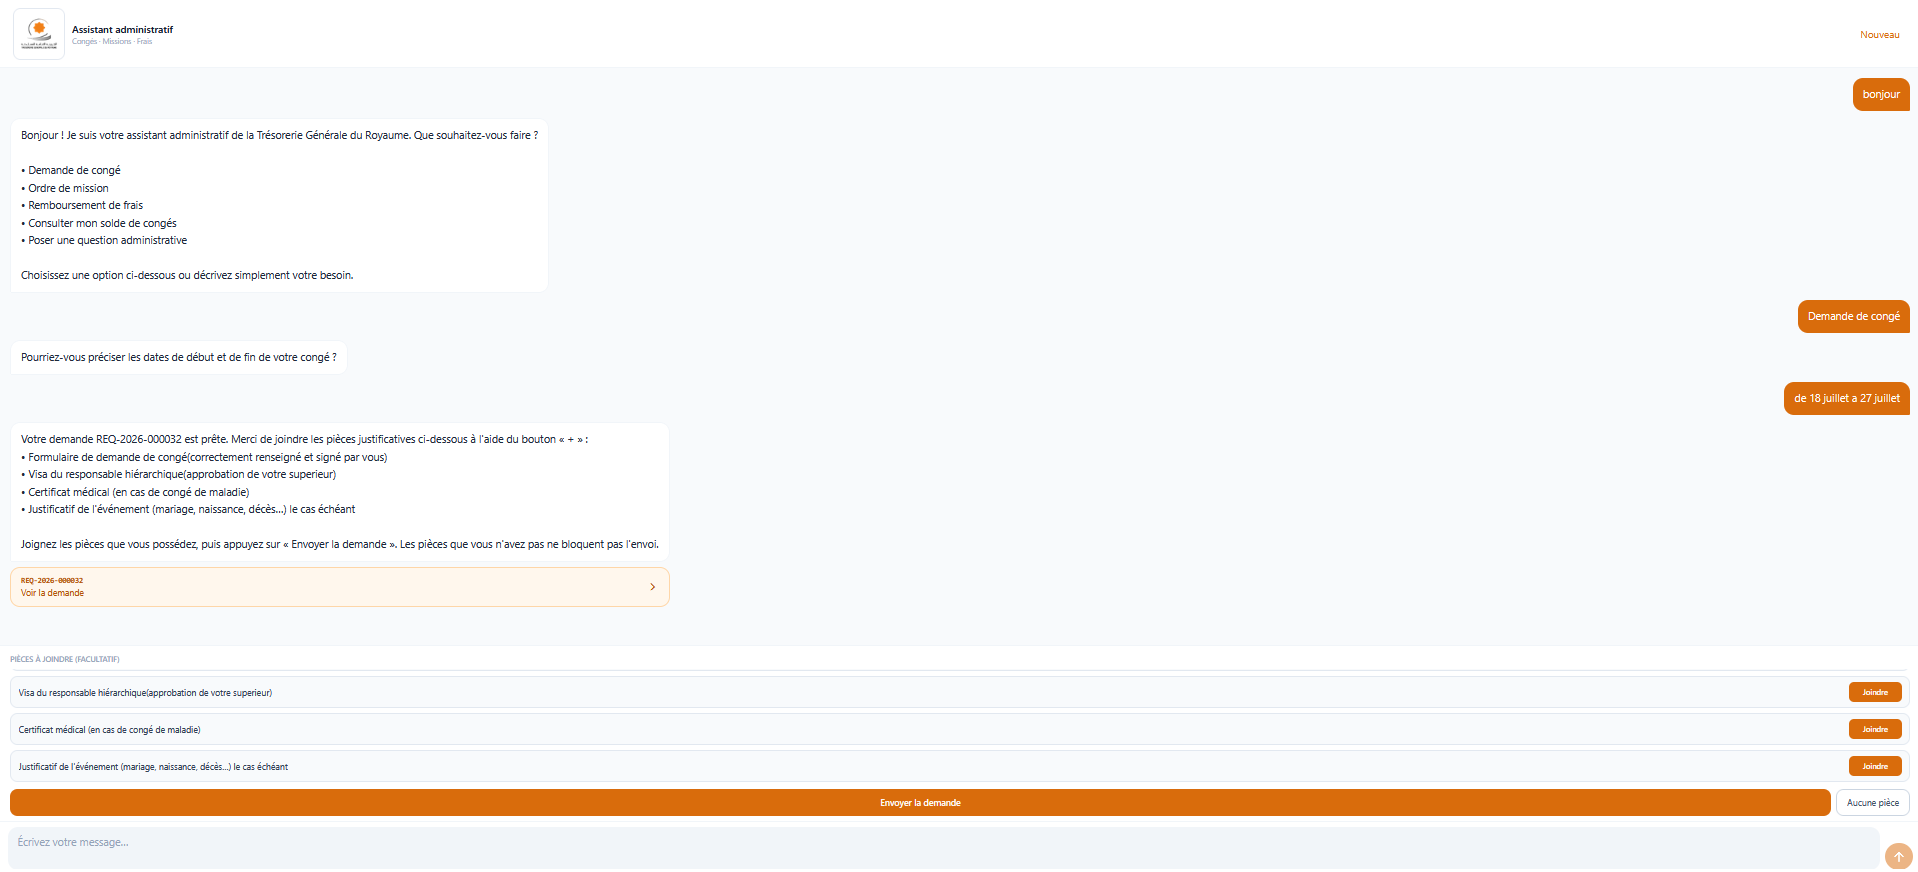
\includegraphics[width=0.86\linewidth]{mobile-assistant.png}
\caption{Application employé : assistant en cours de conversation}
\label{fig:massistant}
\end{figure}

Lorsque l'agent choisit plutôt \emph{obtenir une information}, l'assistant répond
à ses questions administratives en s'appuyant sur le corpus réglementaire et en
\textbf{citant les textes applicables} (figure~\ref{fig:minfo}) : cet écran
illustre la fonction d'\textbf{information} du système, complémentaire du guichet
de demandes.

\begin{figure}[H]
\centering
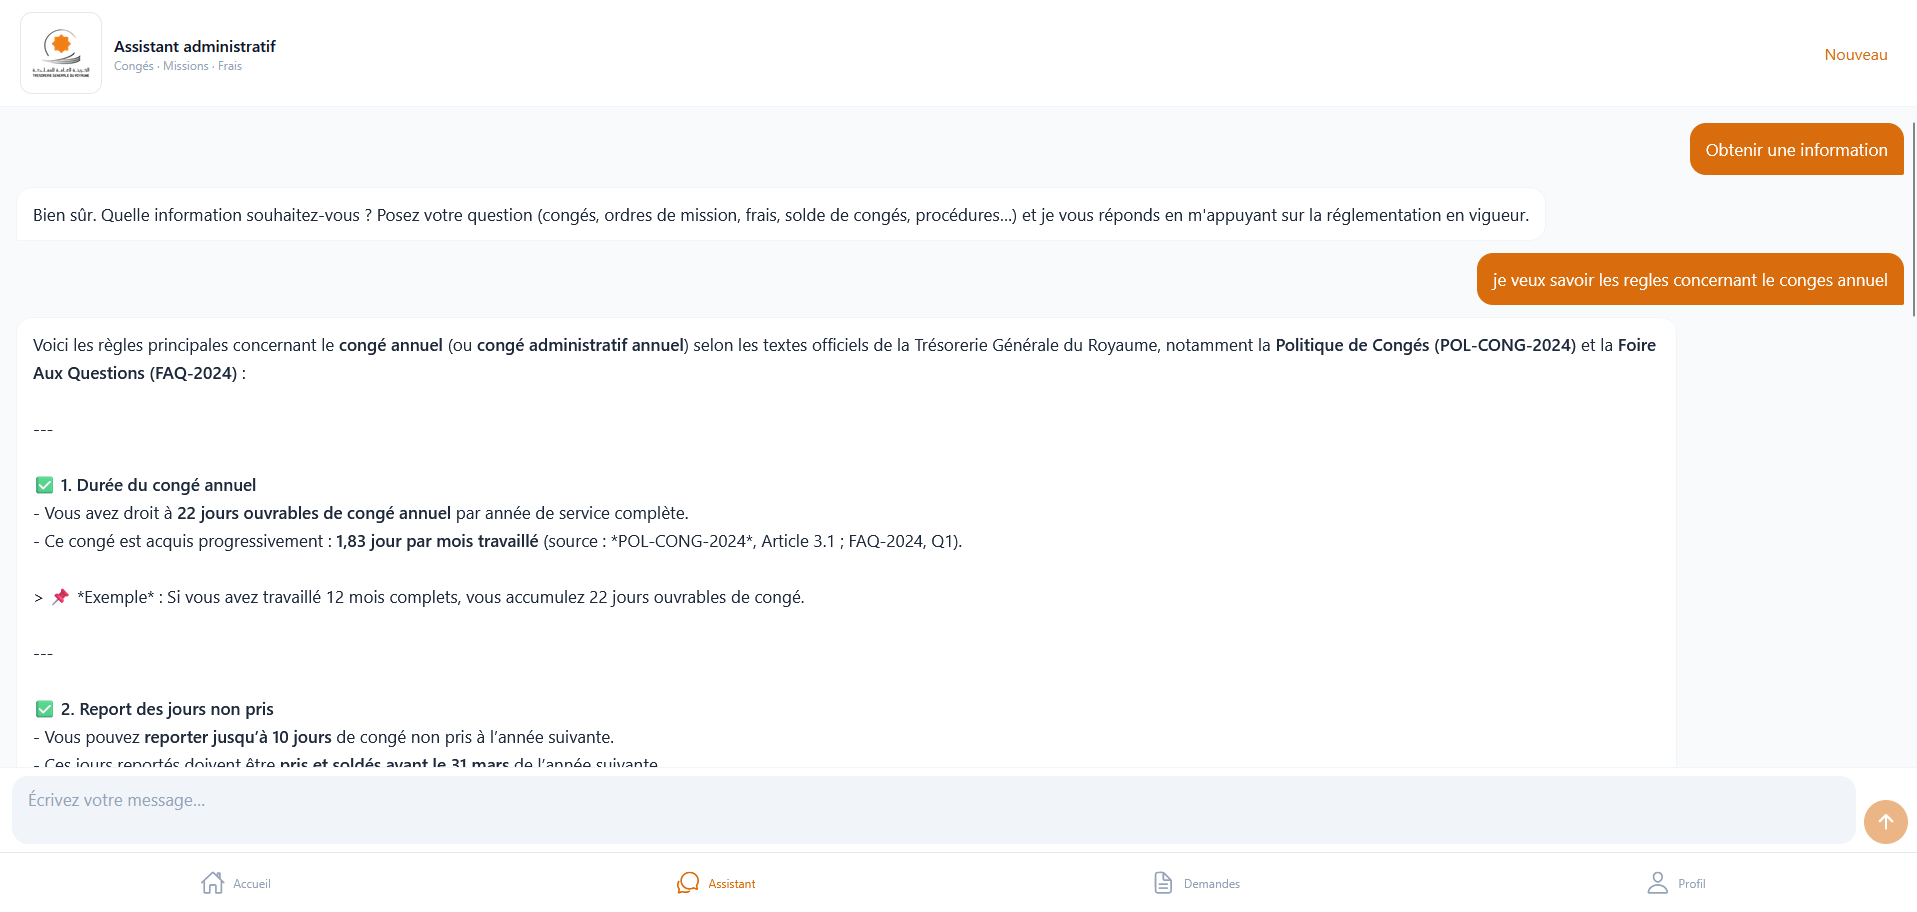
\includegraphics[width=0.95\linewidth]{information-part.png}
\caption{Application employé : réponse sourcée à une question administrative (fonction d'information)}
\label{fig:minfo}
\end{figure}

L'onglet \textbf{Demandes} (figure~\ref{fig:mdemandes}) liste les demandes de
l'employé et leur statut.

\begin{figure}[H]
\centering
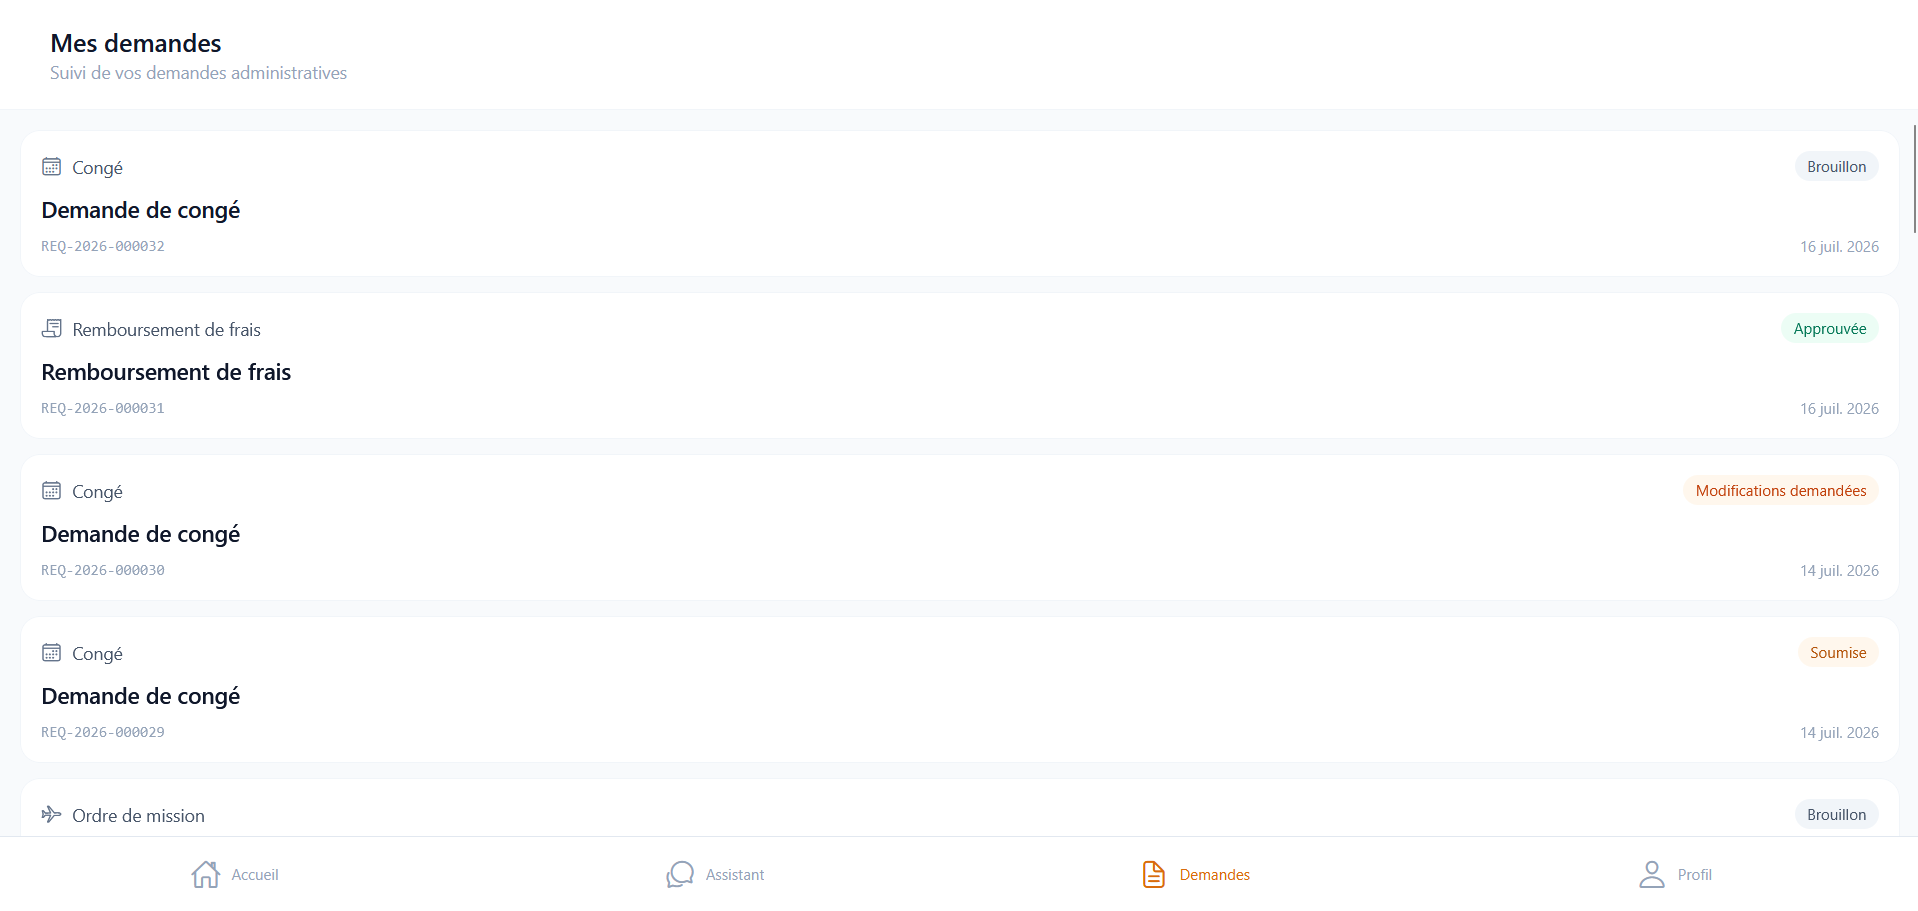
\includegraphics[width=0.86\linewidth]{mobile-demandes.png}
\caption{Application employé : liste des demandes}
\label{fig:mdemandes}
\end{figure}

Enfin, le \textbf{Profil} (figure~\ref{fig:mprofil}) présente l'identité, le
solde de congés et la déconnexion.

\begin{figure}[H]
\centering
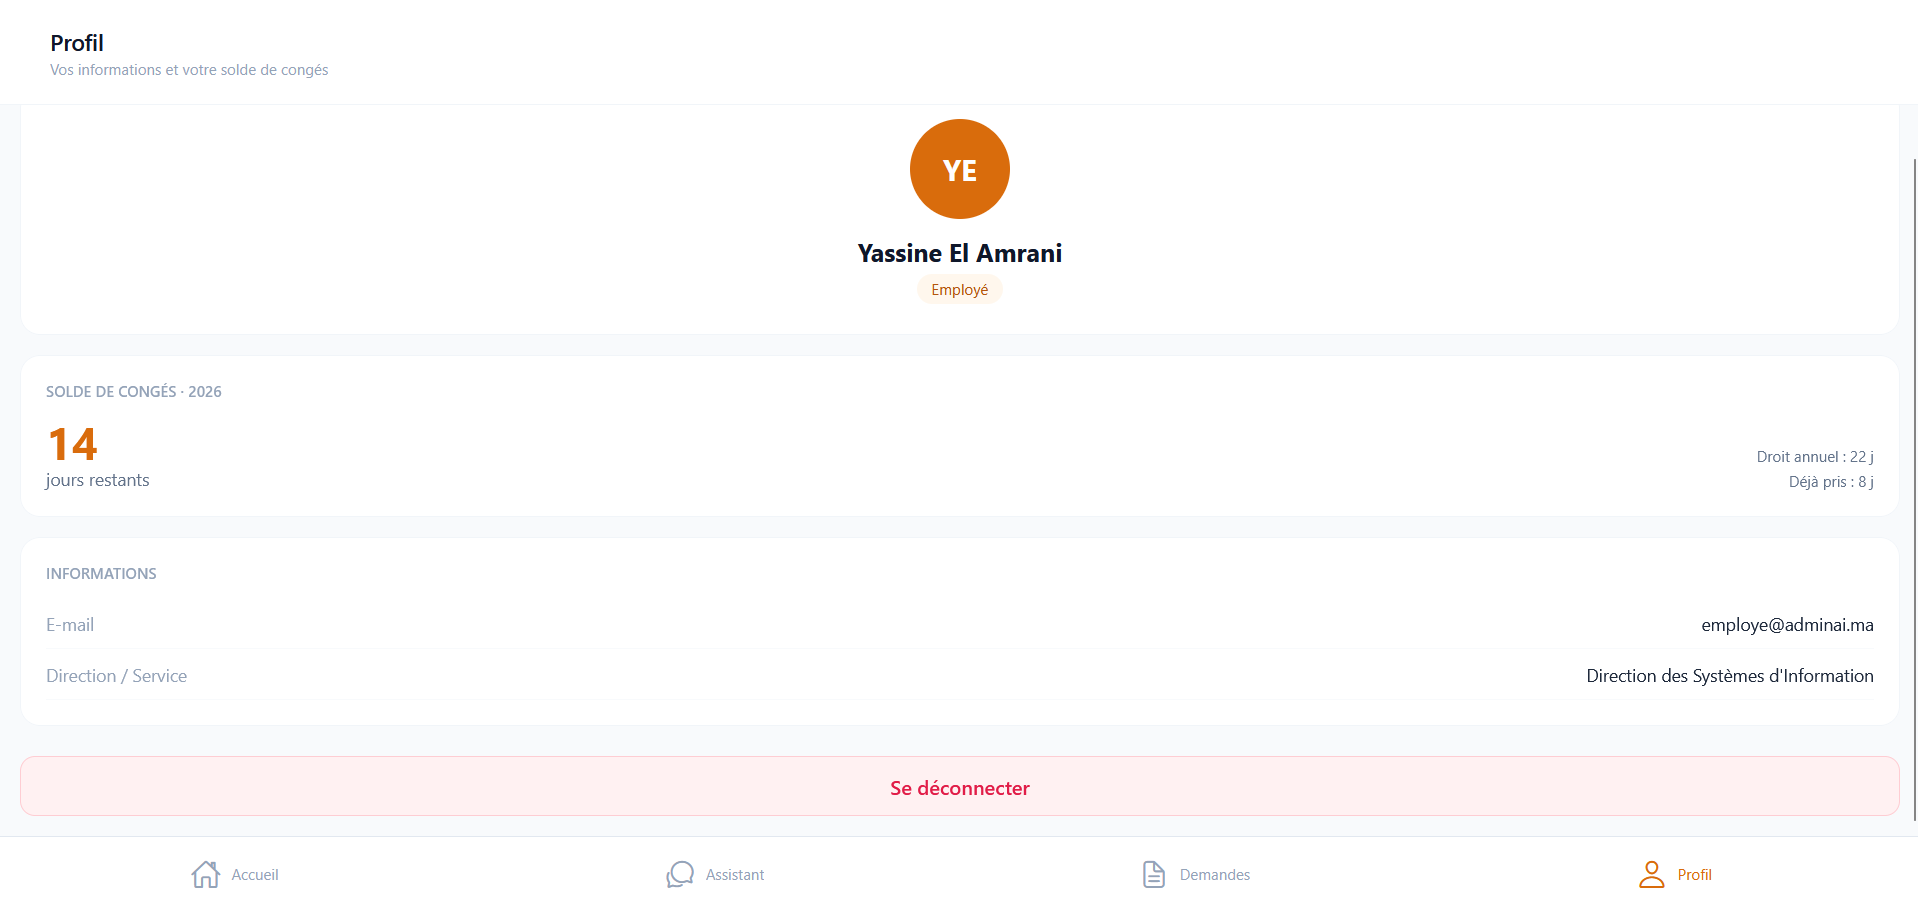
\includegraphics[width=0.86\linewidth]{mobile-profil.png}
\caption{Application employé : profil et solde de congés}
\label{fig:mprofil}
\end{figure}

\section{Tableau de bord des responsables}
Le tableau de bord web offre l'authentification (figure~\ref{fig:dconnexion}),
une vue d'ensemble statistique (figure~\ref{fig:dtableau}), la file des demandes
(figure~\ref{fig:ddemandes}), le détail complet d'une demande avec son analyse IA
(figure~\ref{fig:ddetail}), l'annuaire des employés (figure~\ref{fig:demployes})
et la gestion des notifications (figure~\ref{fig:dnotif}).

\begin{figure}[H]
\centering
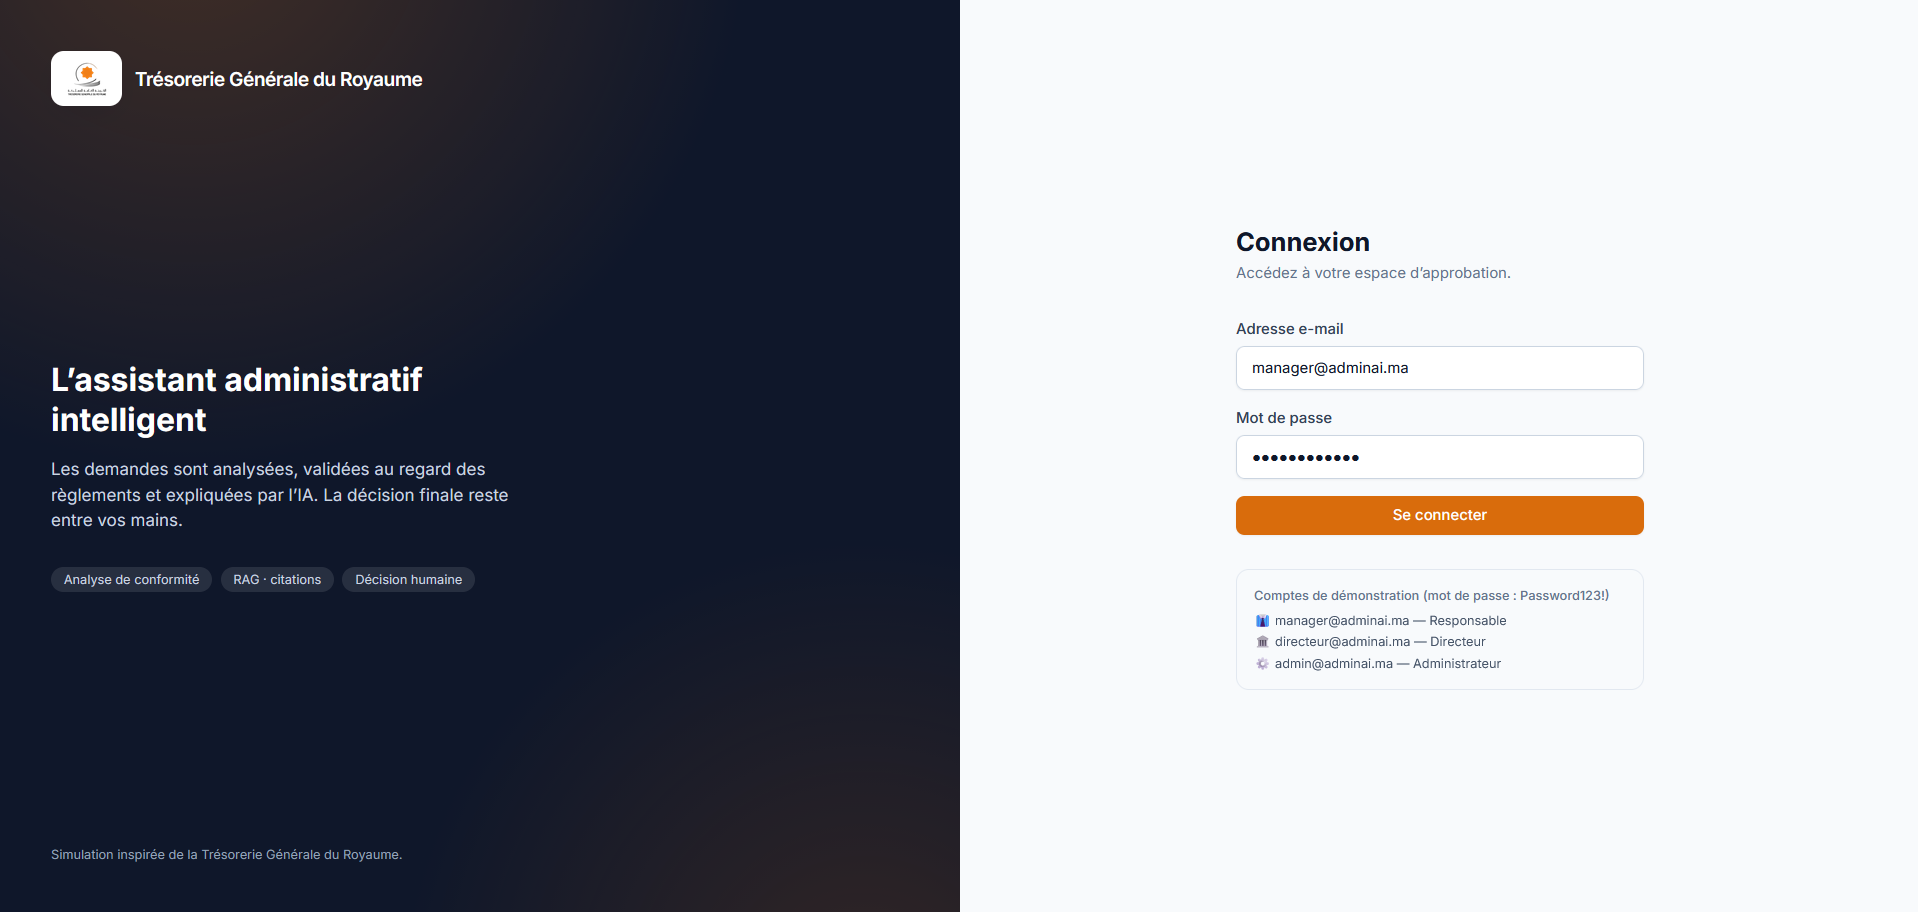
\includegraphics[width=0.95\linewidth]{dashboard-connexion.png}
\caption{Tableau de bord : page de connexion}
\label{fig:dconnexion}
\end{figure}

\begin{figure}[H]
\centering
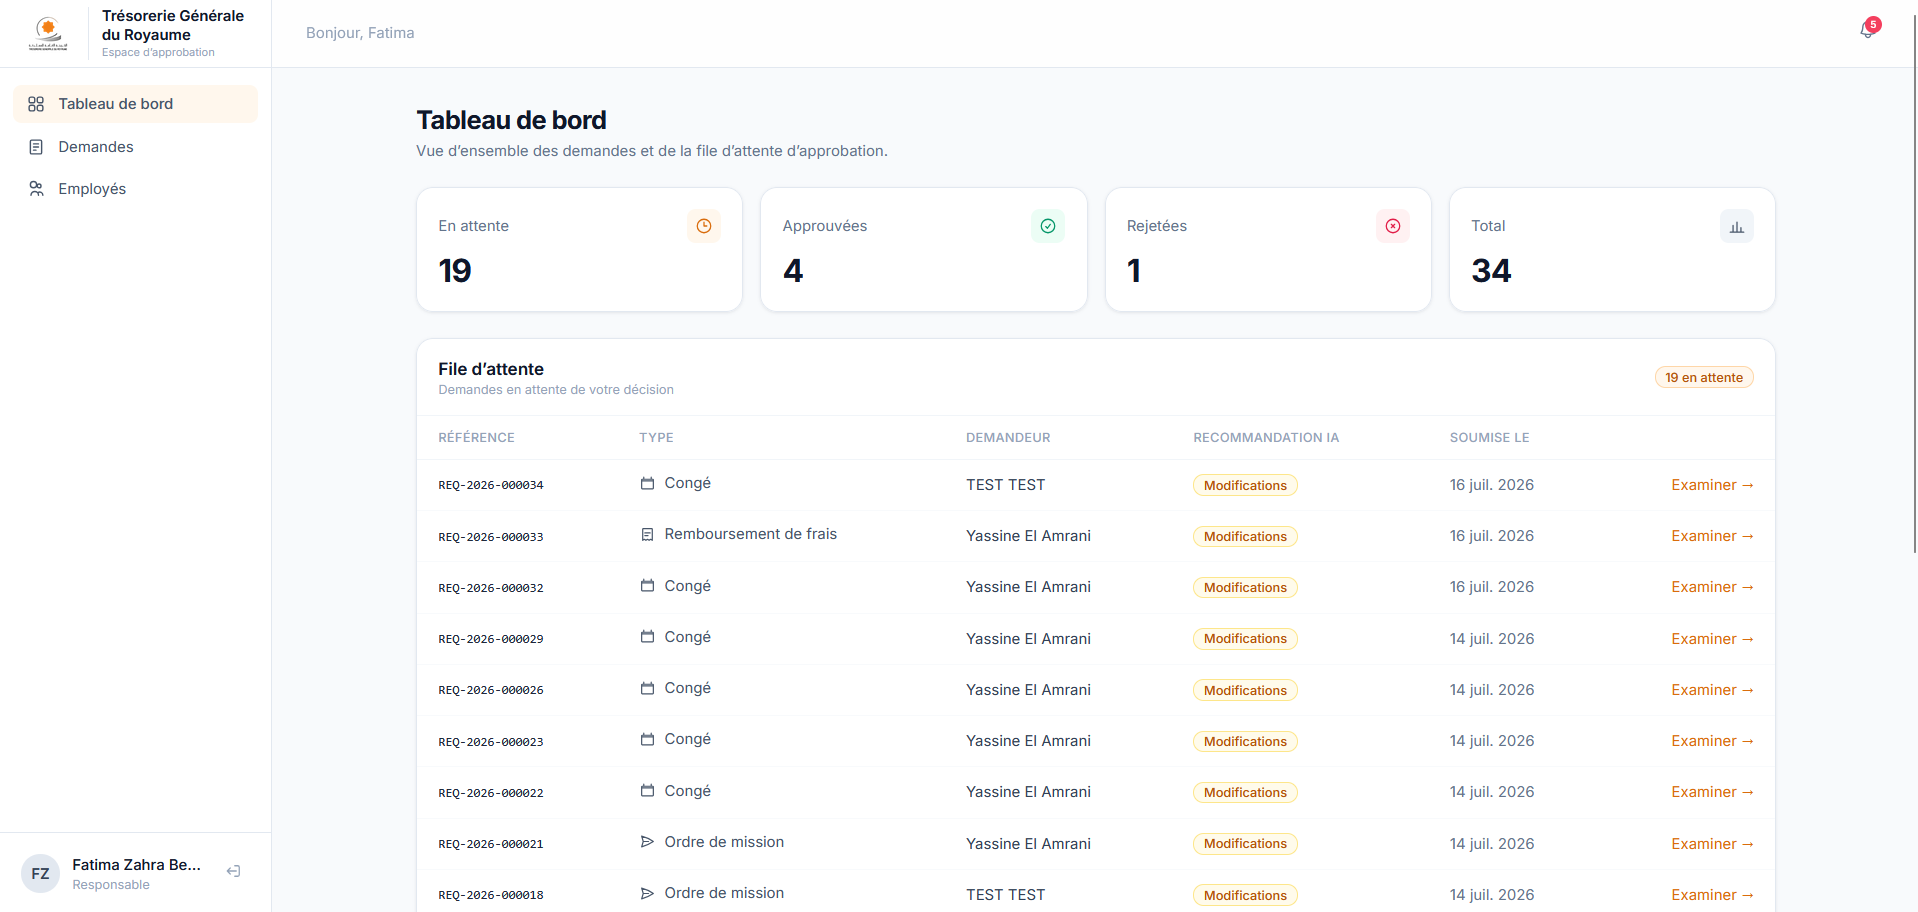
\includegraphics[width=0.95\linewidth]{dashboard-tableau.png}
\caption{Tableau de bord : vue d'ensemble et file d'attente}
\label{fig:dtableau}
\end{figure}

\begin{figure}[H]
\centering
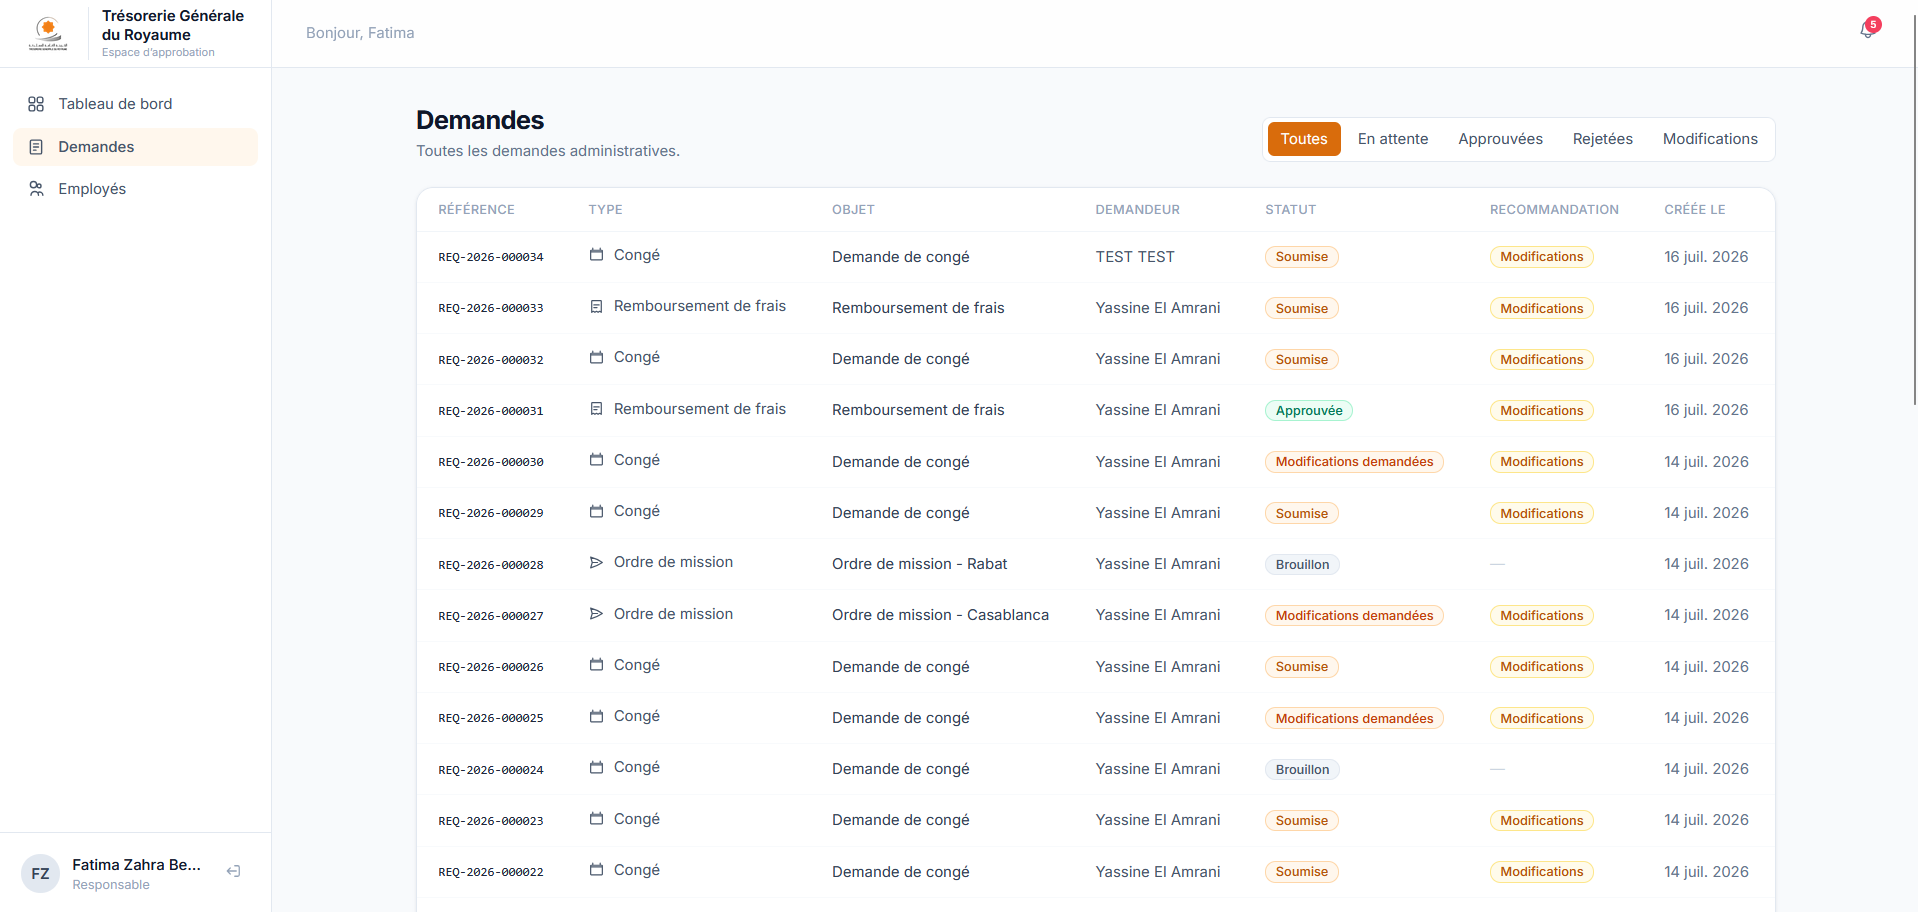
\includegraphics[width=0.95\linewidth]{dashboard-demandes.png}
\caption{Tableau de bord : liste des demandes}
\label{fig:ddemandes}
\end{figure}

Le détail d'une demande (figure~\ref{fig:ddetail}) réunit les informations
saisies, les pièces jointes téléchargeables, l'analyse de l'IA (recommandation,
statut de conformité, résumé), la zone de décision, un champ pour interroger l'IA
et la chronologie de la demande.

\begin{figure}[H]
\centering
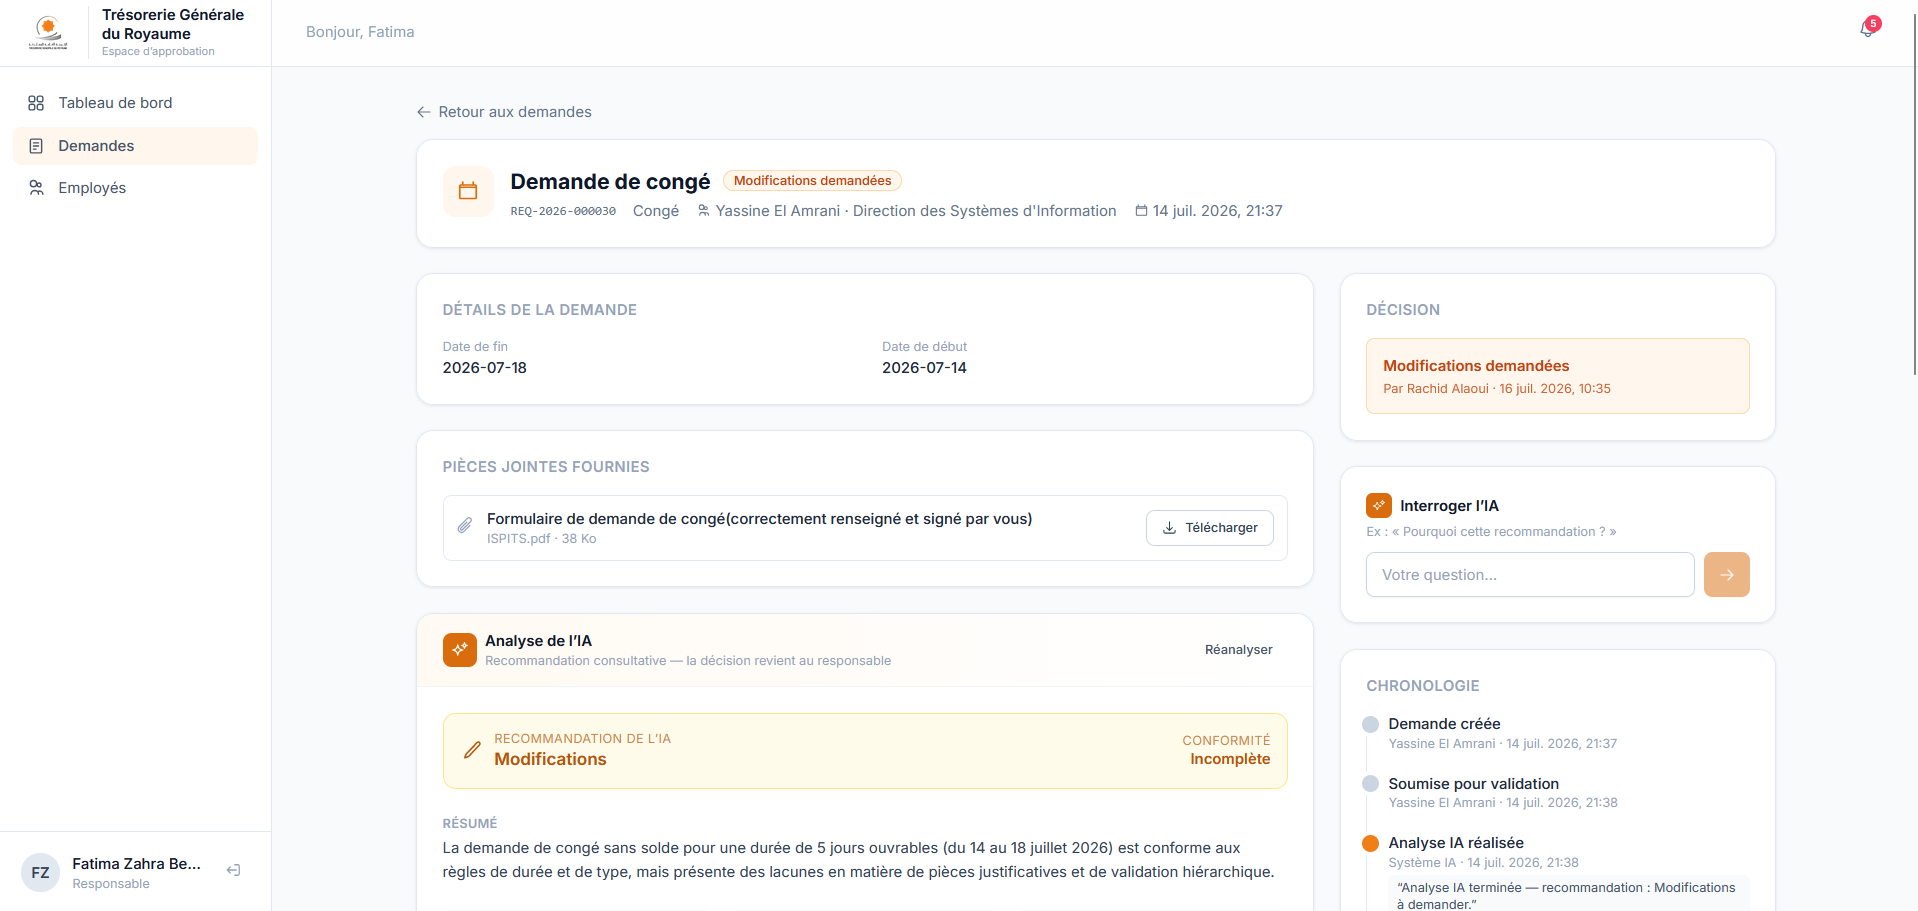
\includegraphics[width=0.95\linewidth]{dashboard-detail.png}
\caption{Tableau de bord : détail d'une demande et analyse IA}
\label{fig:ddetail}
\end{figure}

\begin{figure}[H]
\centering
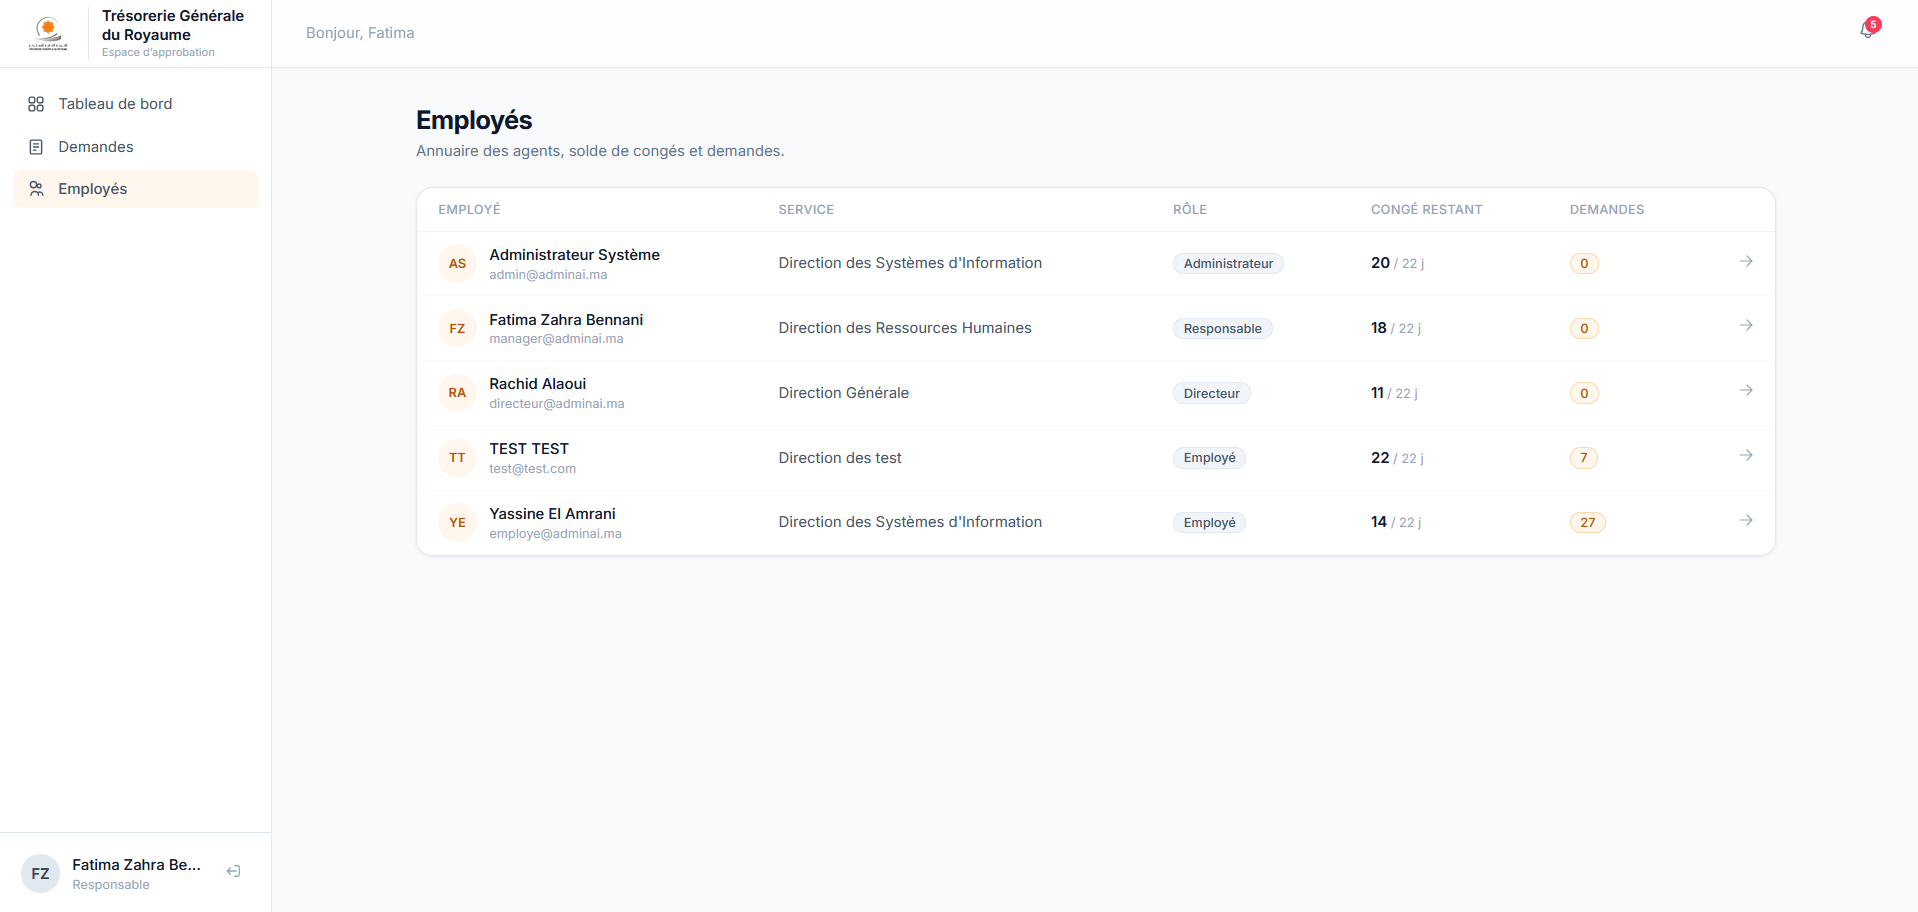
\includegraphics[width=0.95\linewidth]{dashboard-employes.png}
\caption{Tableau de bord : annuaire des employés}
\label{fig:demployes}
\end{figure}

\begin{figure}[H]
\centering
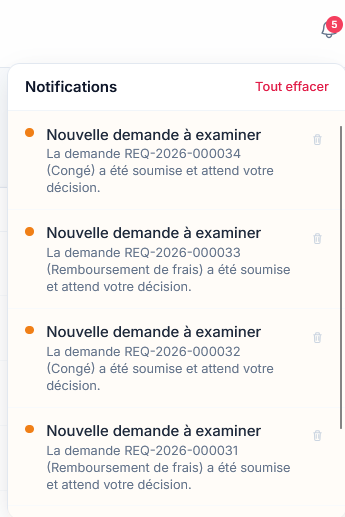
\includegraphics[width=0.95\linewidth]{dashboard-notifications.png}
\caption{Tableau de bord : centre de notifications}
\label{fig:dnotif}
\end{figure}

\section{Sécurité}
La sécurité repose sur une authentification JWT \emph{stateless}, le hachage des
mots de passe (BCrypt), une autorisation par rôle au niveau des méthodes, une
restriction stricte des chemins publics, une configuration CORS maîtrisée et une
traçabilité assurée par un journal d'audit et un fil d'événements par demande.

% =====================================================================
%  CHAPITRE 6
% =====================================================================
\chapter{Bilan du stage}

\section{Apports du stage}
Sur le \textbf{plan professionnel}, ce stage a permis de conduire un projet
logiciel complet, de l'analyse du besoin jusqu'à la livraison d'une solution
conteneurisée, en intégrant des technologies d'intelligence artificielle
récentes (LLM, embeddings, bases vectorielles) dans une architecture rigoureuse.
Sur le \textbf{plan personnel}, il a renforcé l'autonomie, la rigueur, la gestion
du temps et la capacité à résoudre des problèmes complexes de manière méthodique.

D'un point de vue quantitatif, le travail réalisé se traduit par un ensemble
cohérent de composants, dont quelques repères sont donnés au
tableau~\ref{tab:chiffres}.

\begin{table}[H]
\centering
\begin{tabularx}{\linewidth}{X r}
\toprule
\rowcolor{gHead}\thd{Élément} & \thd{Nombre} \\
\midrule
Applications livrées (backend, tableau de bord, application employé) & 3 \\
\rowcolor{gBand}
Entités persistantes du domaine & 12 \\
Migrations de base de données (Flyway) & 5 \\
\rowcolor{gBand}
Services conteneurisés (Docker Compose) & 5 \\
Dimension des vecteurs d'embeddings (bge-m3) & 1024 \\
\rowcolor{gBand}
Découpage RAG : taille / chevauchement (caractères) & 3600 / 650 \\
\bottomrule
\end{tabularx}
\caption{Quelques chiffres du projet réalisé}
\label{tab:chiffres}
\end{table}

\section{Compétences et outils mis en oeuvre}
Le stage a consolidé la maîtrise de plusieurs outils et technologies :
développement backend (Spring Boot, Spring Security, JPA), bases de données
relationnelles et vectorielles (PostgreSQL, pgvector), intégration de modèles de
langage et pipeline RAG (LangChain4j, Ollama), développement front-end web
(Angular) et mobile (React Native / Expo), ainsi que la conteneurisation
(Docker) et la modélisation (UML).

\section{Regard critique sur la formation académique}
La formation dispensée à l'ESI a constitué un socle solide pour aborder ce
projet, notamment en génie logiciel, en bases de données et en méthodes de
conception. Le stage a mis en évidence la complémentarité entre la
\textbf{théorie} et la \textbf{pratique} : si les fondamentaux étaient acquis,
leur mise en oeuvre sur un cas réel a exigé un effort d'adaptation, en
particulier sur les technologies récentes d'intelligence artificielle
générative, moins couvertes par les enseignements et largement approfondies en
autonomie durant le stage. Cette articulation confirme l'importance des projets
pratiques dans la consolidation des acquis.

\section{Difficultés rencontrées}
Plusieurs difficultés techniques ont jalonné le projet :

\begin{itemize}
  \item la \textbf{fiabilité des sorties du LLM}, résolue par une extraction
  tolérante du JSON produit ;
  \item la \textbf{qualité de la recherche en français}, ajustée via le choix du
  modèle d'embeddings et le paramétrage du découpage ;
  \item l'\textbf{exactitude des dates}, garantie par un contrôle explicite qui
  refuse les dates passées ;
  \item la \textbf{distinction information / pièce manquante}, traitée de manière
  déterministe côté serveur ;
  \item la \textbf{coordination des services conteneurisés} (base, moteur
  d'embeddings, téléchargement du modèle, backend).
\end{itemize}

% =====================================================================
%  CONCLUSION
% =====================================================================
\chapter*{Conclusion}
\addcontentsline{toc}{chapter}{Conclusion}
\markboth{Conclusion}{Conclusion}

Ce stage d'études a permis de concevoir et de réaliser un agent administratif
intelligent complet, de l'application web progressive de l'employé au tableau de bord de
validation, en passant par un backend robuste et un pipeline RAG opérationnel. La
solution répond à la problématique posée : elle assiste l'agent dans la
formulation de ses demandes en langage naturel, vérifie leur conformité au regard
d'un corpus réglementaire et fournit au valideur une recommandation explicable et
sourcée, sans se substituer à la décision humaine.

Au regard des objectifs initiaux, le stage peut être considéré comme
\textbf{réussi} : l'ensemble des fonctionnalités visées a été réalisé et vérifié.
Il a par ailleurs apporté une orientation professionnelle plus précise, en
confirmant l'intérêt du stagiaire pour le génie logiciel et l'ingénierie des
systèmes à base d'intelligence artificielle. Plusieurs perspectives d'évolution
se dégagent : recherche hybride (vectorielle et lexicale), notifications en temps
réel, tableaux de bord analytiques, enrichissement et versionnement du corpus, et
évaluation systématique de la qualité des réponses de l'IA en vue d'une
industrialisation.

% =====================================================================
%  BIBLIOGRAPHIE
% =====================================================================
\chapter*{Bibliographie / Webographie}
\addcontentsline{toc}{chapter}{Bibliographie / Webographie}
\markboth{Bibliographie}{Bibliographie}

\begin{thebibliography}{99}
\bibitem{tgr} Trésorerie Générale du Royaume. \emph{Portail officiel}.
\newblock \url{https://www.tgr.gov.ma/} (consulté en 2026).
\bibitem{mef} Ministère de l'Économie et des Finances (Maroc).
\emph{La Trésorerie Générale du Royaume}.
\newblock \url{https://www.finances.gov.ma/}
\bibitem{rag} P. Lewis et al. \emph{Retrieval-Augmented Generation for
Knowledge-Intensive NLP Tasks}. 2020.
\newblock \url{https://arxiv.org/abs/2005.11401}
\bibitem{transformer} A. Vaswani et al. \emph{Attention Is All You Need}. 2017.
\newblock \url{https://arxiv.org/abs/1706.03762}
\bibitem{sbert} N. Reimers, I. Gurevych. \emph{Sentence-BERT: Sentence Embeddings
using Siamese BERT-Networks}. 2019.
\newblock \url{https://arxiv.org/abs/1908.10084}
\bibitem{springboot} \emph{Spring Boot Reference Documentation}.
\newblock \url{https://docs.spring.io/spring-boot/}
\bibitem{langchain4j} \emph{LangChain4j Documentation}.
\newblock \url{https://docs.langchain4j.dev/}
\bibitem{pgvector} \emph{pgvector : Open-source vector similarity search for
Postgres}.
\newblock \url{https://github.com/pgvector/pgvector}
\bibitem{bgem3} BAAI. \emph{BGE-M3 : Multilingual embedding model}.
\newblock \url{https://huggingface.co/BAAI/bge-m3}
\bibitem{angular} \emph{Angular Documentation}.
\newblock \url{https://angular.dev/}
\bibitem{expo} \emph{Expo Documentation (SDK 57)}.
\newblock \url{https://docs.expo.dev/}
\bibitem{docker} \emph{Docker Compose Documentation}.
\newblock \url{https://docs.docker.com/compose/}
\end{thebibliography}

% =====================================================================
%  ANNEXES
% =====================================================================
\appendix
\chapter{Annexes}

\section{Structure des dossiers du projet}
\begin{lstlisting}[caption={Arborescence (extrait)}]
Project/
|-- backend/            # API Spring Boot (Java 21)
|   `-- src/main/java/com/pfe/adminagent/
|       |-- ai/         # orchestrateur, LLM, analyse
|       |-- rag/        # ingestion, recherche semantique
|       |-- request/    # demandes, pieces jointes, decisions
|       |-- conversation/ leave/ notification/ user/ audit/
|       |-- security/   # JWT, filtres
|       `-- config/     # configuration IA/RAG, securite
|-- dashboard/          # SPA Angular 19 + Tailwind (nginx)
|-- mobile/             # App Expo / React Native
|-- knowledge-base/     # Corpus reglementaire FR (13 documents)
|-- docs/diagrams/      # Diagrammes UML (sources PlantUML)
`-- docker-compose.yml  # Orchestration des services
\end{lstlisting}

\section{Configuration (extrait, hors secrets)}
\begin{lstlisting}[language=bash,caption={Variables d'environnement principales}]
LLM_BASE_URL=https://openrouter.ai/api/v1
LLM_MODEL=qwen/qwen3-30b-a3b
LLM_TEMPERATURE=0.2
EMBEDDING_MODEL=bge-m3
EMBEDDING_DIMENSION=1024
\end{lstlisting}

\section{Organigramme détaillé de la TGR}
\label{ann:orga}
Structure officielle complète, reproduite d'après le portail de la Trésorerie
Générale du Royaume : pour chaque direction centrale, ses divisions et ses
services.

\newcommand{\dir}[1]{\medskip\noindent{\large\bfseries #1}\par\vspace{2pt}}
\newcommand{\dive}[1]{\smallskip\noindent\textbf{#1}}
\newenvironment{svc}{\begin{itemize}[nosep,leftmargin=1.6em,label=\textperiodcentered]}{\end{itemize}}

{\small

\dir{1. Direction de la Recherche, de la Réglementation et de la Coopération Internationale}
\dive{Division de la Réglementation}
\begin{svc}
\item Service de la réglementation des finances de l'État et des collectivités territoriales
\item Service de la réglementation des marchés publics
\item Service de la réglementation des dépenses du personnel
\item Service de la réglementation et de la normalisation comptable
\end{svc}
\dive{Division de la Recherche et des Études}
\begin{svc}
\item Service de la recherche
\item Service des manuels de procédures
\item Service de la documentation
\item Service de la communication
\end{svc}
\dive{Division de la Coopération Internationale}
\begin{svc}
\item Service de la coopération en matière des finances de l'État et des collectivités territoriales
\item Service de la coopération en matière de marchés publics
\item Service de la coopération comptable
\end{svc}

\dir{2. Direction des Finances Publiques}
\dive{Division des Finances de l'État}
\begin{svc}
\item Service du suivi des recettes de l'État
\item Service du suivi des dépenses de l'État
\item Service de la réforme budgétaire et des relations avec les ministères
\item Service des affaires juridiques
\end{svc}
\dive{Division des Finances des Collectivités Territoriales et des Autres Organismes}
\begin{svc}
\item Service du suivi des recettes des collectivités territoriales
\item Service du suivi des dépenses des collectivités territoriales
\item Service des relations avec les collectivités territoriales
\item Service du recouvrement des créances des autres organismes
\end{svc}
\dive{Division de la Dette Publique}
\begin{svc}
\item Service de la gestion de la dette publique
\item Service des dépôts au trésor
\item Service du suivi de l'activité bancaire
\end{svc}
\dive{Division des Systèmes de Gestion Intégrée}
\begin{svc}
\item Service de la gestion intégrée des recettes
\item Service de la gestion intégrée des dépenses
\item Service de la gestion intégrée de la dette
\item Service de la dématérialisation des marchés publics
\end{svc}

\dir{3. Direction des Dépenses du Personnel}
\dive{Division de la Paie du Personnel de l'État}
\begin{svc}
\item Service de la paie du personnel de l'État
\item Service des prélèvements sur la paie du personnel de l'État
\item Service des relations avec les trésoreries ministérielles
\item Service de la gestion intégrée des dépenses du personnel
\end{svc}
\dive{Division de la Paie du Personnel des Collectivités Territoriales et des Autres Organismes}
\begin{svc}
\item Service de la paie du personnel des collectivités territoriales
\item Service de la paie du personnel des autres organismes
\item Service des prélèvements sur la paie du personnel des collectivités territoriales et des autres organismes
\item Service des relations avec les collectivités territoriales et les autres organismes
\end{svc}
\dive{Division du Règlement des Dépenses du Personnel et de la Comptabilité}
\begin{svc}
\item Service de la liquidation de la paie
\item Service du contrôle de la paie
\item Service des oppositions juridiques et du recouvrement sur la rémunération du personnel
\item Service du règlement et de la comptabilité de la paie du personnel
\end{svc}

\dir{4. Direction des Comptes Publics}
\dive{Division de la Centralisation des Comptes de l'État et des Collectivités Territoriales}
\begin{svc}
\item Service de la centralisation des comptes de l'État
\item Service du suivi des comptes des collectivités territoriales
\item Service des états financiers et des lois de règlement
\item Service de la gestion intégrée du système comptable
\end{svc}
\dive{Division du Suivi de la Reddition des Comptes Publics}
\begin{svc}
\item Service de l'examen et du suivi de la responsabilité des comptables
\item Service du contrôle de la qualité comptable
\item Service du suivi de la reddition des comptes de l'État et des collectivités territoriales
\end{svc}
\dive{Division des Statistiques des Finances de l'État et des Collectivités Territoriales}
\begin{svc}
\item Service des statistiques des finances de l'État
\item Service des statistiques des finances des collectivités territoriales
\item Service des statistiques des dépenses du personnel de l'État et des collectivités territoriales
\item Service du suivi des flux de trésorerie de l'État et des collectivités territoriales
\end{svc}

\dir{5. Direction des Ressources et du Système d'Information}
\dive{Division des Ressources Humaines}
\begin{svc}
\item Service de la gestion des ressources humaines
\item Service de la gestion prévisionnelle des ressources humaines
\item Service de la formation
\item Service de l'action sociale
\end{svc}
\dive{Division du Budget et de la Logistique}
\begin{svc}
\item Service du budget
\item Service des achats
\item Service de la logistique
\item Service de la gestion du patrimoine
\end{svc}
\dive{Division du Développement Informatique \textnormal{(division du stage)}}
\begin{svc}
\item Service de l'assistance à la maîtrise d'ouvrage
\item Service de l'architecture et de la conception
\item Service du développement
\item Service du paramétrage et de l'intégration
\end{svc}
\dive{Division de l'Exploitation Informatique}
\begin{svc}
\item Service de la gestion des plateformes
\item Service des applications et des données
\item Service des réseaux et télécommunications
\item Service de la bureautique
\item Service de la sécurité informatique
\end{svc}

\dir{6. Direction du Contrôle, de l'Audit et de l'Inspection}
\dive{Division du contrôle interne}
\begin{svc}
\item Service de la gestion des risques
\item Service du contrôle interne
\item Service du management de la qualité
\end{svc}
\dive{Division du contrôle de gestion}
\begin{svc}
\item Service de la mise en oeuvre du contrôle de gestion
\item Service du pilotage des programmes d'action
\item Service de l'analyse et du suivi de la performance
\end{svc}
\dive{Division de l'Audit et de l'Inspection}
\begin{svc}
\item Service de l'audit interne
\item Service de l'audit de la capacité de gestion des ordonnateurs
\item Service de l'inspection des comptables de l'État
\item Service de l'inspection des comptables des collectivités territoriales
\end{svc}

}

\end{document}
